\documentclass[compress, aspectratio=169,usepdftitle=false]{beamer}
%\setbeameroption{show notes on second screen=left}
\usepackage[utf8]{inputenc}
\usepackage{braket}
\newcommand{\identity}[0]{\mathbf{1}}
\newcommand{\Op}[1]{\ensuremath{\mathsf{\hat{#1}}}}
\def\mat#1{\hat{#1}}
\def\half{ \frac{1}{2}}
\newcommand{\TildeOp}[1]{\ensuremath{\mathsf{\tilde{#1}}}}
\newcommand{\vectorize}{\operatorname{vec}}
\newcommand{\Abs}[1]{\left|#1\right|}
\newcommand{\AbsSq}[1]{\left|#1\right|^2}
\newcommand{\Norm}[1]{\left\lVert#1\right\rVert}
\newcommand{\NormSq}[1]{\Norm{#1}^2}
\newcommand{\tr}{\mathsf{tr}}
\newcommand{\Tr}{\mathsf{tr}}
\newcommand{\SU}{\ensuremath{\text{SU}}}
\newcommand{\ketbra}[2]{\ket{#1}\!\bra{#2}}
\newcommand{\mirror}{\text{mirror}}
\newcommand{\tgt}{\text{tgt}}
\newcommand{\pop}{\operatorname{pop}}
\newcommand{\dd}{\mathsf{d}}
\newcommand{\ii}{\mathsf{i}}
\newcommand{\Integers}{\mathbb{Z}}
\newcommand{\norm}{\operatorname{norm}}
\renewcommand{\Re}{\mathsf{Re}}
\renewcommand{\Im}{\mathsf{Im}}
\newcommand{\partdifquo}[2][{}]{\frac{\partial #1}{\partial #2}}
\newcommand{\Reals}{\mathbb{R}}
\newcommand{\Complex}{\mathbb{C}}
\newcommand{\Liouvillian}{\mathcal{L}}
\newcommand{\TimeOrder}{\mathcal{T}}
\newcommand{\SigmaX}{\Op{\sigma}_x}
\newcommand{\SigmaY}{\Op{\sigma}_y}
\newcommand{\SigmaZ}{\Op{\sigma}_z}
\newcommand{\SigmaPlus}{\Op{\sigma}_{\!+}}
\newcommand{\SigmaMinus}{\Op{\sigma}_{\!-}}
\usepackage{textcomp} % provides \textmu
\usepackage{tikz}
\usepackage{hyperref}
\usepackage{fontawesome}
\usetikzlibrary{shapes, arrows.meta, calc, decorations.pathmorphing, backgrounds, positioning}

\usepackage{amsmath, xparse, letltxmacro}
\LetLtxMacro{\oldunderbrace}{\underbrace}

\DeclareDocumentCommand{\underbrace}{d<> m e{_}}{%
  \IfValueTF{#1}{% IF <overlay-specification> given
    % using global onlside flag, cf. p82 beamer manual v3.59
    \oldunderbrace{#2\onslide<#1>}_{#3}\onslide%
  }{% ELSE
    \oldunderbrace{#2}_{#3}
  }%
}%

%% Notes on screenshots:
%
% - Make sure ``Reduce Transparency'' in the Accessibility settings (Display) is off
% - Size window to 1270 x 625 (2540 x 1250 retina)
%   - if no title on slide: increase height +41 to 666  (1332 retina)
% - Take screenshots at retina resolution
% - Terminal (iTerm) is at standard size +5 font size increases
% - JupyterLab in Arc – for slide without title:
%   - total window size 1364 x 800
%   - ``Simple Interface'' (View Menu)
%   - ``Presentation Mode'' (View Menu)
%   - No status bar (View Menu)


%%%%%%%%%%%%%%%%%%%%%%%%%%%%%%%%%%%%%%%%%%%%%%%%%%%%%%%%%%%%%%%%%%%%%%%%%%%%%%%%
% This theme is for ARL slides in widescreen (16:9) format
%
% Usage: use beamer class
%
%     \documentclass[12pt, compress, aspectratio=169]{beamer}
%
% and e.g.
%
%     %%%%%%%%%%%%%%%%%%%%%%%%%%%%%%%%%%%%%%%%%%%%%%%%%%%%%%%%%%%%%%%%%%%%%%%%%%%%%%%%
% This theme is for ARL slides in widescreen (16:9) format
%
% Usage: use beamer class
%
%     \documentclass[12pt, compress, aspectratio=169]{beamer}
%
% and e.g.
%
%     %%%%%%%%%%%%%%%%%%%%%%%%%%%%%%%%%%%%%%%%%%%%%%%%%%%%%%%%%%%%%%%%%%%%%%%%%%%%%%%%
% This theme is for ARL slides in widescreen (16:9) format
%
% Usage: use beamer class
%
%     \documentclass[12pt, compress, aspectratio=169]{beamer}
%
% and e.g.
%
%     \input{arlwide_theme/theme.tex}
%     \title[Optimal pulse schemes for atom interferometry]{%
%       Optimal pulse schemes \\for high-precision atom interferometry}
%     \author[Michael Goerz (goerz@stanford.edu)]{%
%       {\bf M. Goerz}$^1$, P. Kunz$^1$, M. Kasevich$^2$, V. Malinovsky$^1$
%     }
%     \institute[\protect{\includegraphics[height=5pt]{images/arl}}]{%
%       $^1$U.S. Army Research Lab, $^2$Stanford University
%     }
%     \date{August 23, 2018}
%
% in the header of the tex file. Make sure to disable any footer on the
% titlepage:
%
%     {%  Title page
%       \setbeamertemplate{footline}{}
%       \frame{\titlepage}
%     }
%     \addtocounter{framenumber}{-1}
%
% NOTE: for documentation of how to modify templates, in addition to the Beamer
% user guide, use
% http://www.cpt.univ-mrs.fr/~masson/latex/Beamer-appearance-cheat-sheet.pdf
%
%%%%%%%%%%%%%%%%%%%%%%%%%%%%%%%%%%%%%%%%%%%%%%%%%%%%%%%%%%%%%%%%%%%%%%%%%%%%%%%%
\usepackage{tikz}
\usetikzlibrary{calc}
\usetikzlibrary{positioning}


%%%%%%%%%%%%%%%%%%%%%%%%%%%%%% Grid %%%%%%%%%%%%%%%%%%%%%%%%%%%%%%%%%%%%%%%%%%%%
% Set up grid for absolute text positioning (page size = 16 x 9 cm)
\usepackage[absolute, overlay]{textpos}
% \usepackage[absolute, overlay, showboxes]{textpos} % (`showboxes` for debugging)
\textblockorigin{0cm}{0cm} % The grid guides start from top left
\setlength{\TPHorizModule}{1cm} % Units are 1 cm ...
\setlength{\TPVertModule}{1cm} % ... and y coordinates point down
% Now you can use e.g.:
%    \begin{textblock}{3}(4,2)
%      \dots
%    \end{textblock}
% to place a block 3cm wide, 4cm right and 2cm up from the bottom left corner
%%%%%%%%%%%%%%%%%%%%%%%%%%% Theme Settings %%%%%%%%%%%%%%%%%%%%%%%%%%%%%%%%%%%%%

\definecolor{DarkBlue}{rgb}{0.1,0.1,0.5}
\definecolor{DarkRed}{rgb}{0.75,0.,0.}
\definecolor{Magenta}{rgb}{1.0,0.0,1.0}
\definecolor{Red}{rgb}{0.894,0.102,0.110}
\definecolor{Green}{rgb}{0.302,0.686,0.290}
\definecolor{Blue}{rgb}{0.216,0.494,0.722}
\definecolor{Orange}{rgb}{1.000,0.498,0.000}
\definecolor{Yellow}{rgb}{0.824,0.824,0.082}
\definecolor{Brown}{rgb}{0.651,0.337,0.157}
\definecolor{LightBlue}{rgb}{0.651,0.808,0.890}
\definecolor{Purple}{rgb}{0.596,0.306,0.639}
\definecolor{LightPurple}{rgb}{0.792,0.698,0.839}
\definecolor{Grey}{rgb}{0.600,0.600,0.600}
\definecolor{LightGreen}{rgb}{0.698,0.875,0.541}
\definecolor{LightOrange}{rgb}{0.992,0.749,0.435}
\definecolor{Pink}{rgb}{0.969,0.506,0.749}
\definecolor{Black}{rgb}{0.000,0.000,0.000}
\definecolor{LightRed}{rgb}{0.984,0.604,0.600}
\definecolor{White}{rgb}{1.000,1.000,1.000}

\definecolor{ARLGray25}{rgb}{0.698,0.698,0.698}


%%%%%%%%%%%%%%%%%%%%%%%%%%% Theme Settings %%%%%%%%%%%%%%%%%%%%%%%%%%%%%%%%%%%%%
\usetheme{Berlin}
\useoutertheme{shadow}
\useinnertheme{default}
\setbeamercolor{palette primary}{use=structure,fg=black,bg=black!20!white}
\setbeamercolor{palette secondary}{use=structure,fg=black,bg=black!25!white}
\setbeamercolor{palette tertiary}{use=structure,fg=black,bg=black!30!white}
\setbeamercolor{palette quaternary}{use=structure,fg=black,bg=black!35!white}
\setbeamercolor{sidebar}{use=structure,bg=structure.fg!20!white}
\setbeamercolor{palette sidebar primary}{use=normal text,fg=normal text.fg}
\setbeamercolor{palette sidebar secondary}{use=structure,fg=structure.fg}
\setbeamercolor{palette sidebar tertiary}{use=normal text,fg=normal text.fg}
\setbeamercolor{palette sidebar quaternary}{use=structure,fg=structure.fg}
\setbeamercolor*{titlelike}{parent=palette primary}
\setbeamercolor*{separation line}{}
\setbeamercolor*{fine separation line}{}
\setbeamertemplate{blocks}[rounded][shadow=false]
\setbeamerfont{title}{family*=phv, size*={20}{24}}
\setbeamerfont{author}{family*=phv, size*={12}{14}}
\setbeamerfont{institute}{family*=phv, size*={8.0}{12}}
\setbeamerfont{date}{family*=phv, size*={8.0}{12}}
\setbeamerfont{classification}{family*=phv, size*={3.78}{4.5}}
\setbeamerfont{frametitle}{series=\bfseries, family*=phv, size*={11.34}{14}}
\defbeamertemplate*{title page}{customized}[1][]{%
  \tikz[overlay,remember picture] (current page.south west) rectangle (current page.north east);
  \begin{textblock}{14}(0.0,0.0)
    
\includegraphics[width=\textwidth]{arlwide_theme/arl_devcom_title}
  \end{textblock}
  \begin{textblock}{14}(1,2.75)
    \begin{center}
      \setlength{\baselineskip}{24pt} % cf. height of \setbeamerfont{title}
      {\color{black} \usebeamerfont{title} \inserttitle}
    \end{center}
  \end{textblock}
  \begin{textblock}{14}(1,5.0)
    \begin{center}
      {\color{black} \usebeamerfont{author} \insertauthor}
    \end{center}
  \end{textblock}
  \begin{textblock}{14}(1,6.25)
    \begin{center}
      {\color{black} \usebeamerfont{institute} \insertinstitute}
    \end{center}
  \end{textblock}
  \begin{textblock}{14}(1,7.5)
    \begin{center}
      {\color{black} \usebeamerfont{date} \insertdate}
    \end{center}
  \end{textblock}
}
\setbeamertemplate{background canvas}{%
  % textblock does not work in background canvas, for some reason
  %\tikz[overlay,remember picture] \node[at=(current page.center)]{%
    %\includegraphics[height=\paperheight,width=\paperwidth]
    %{arlwide_theme/titleexample.pdf}};
  \begin{tikzpicture}[remember picture, overlay]
    %%% grid for positioning (debugging)
    %\draw[step=1cm, color=blue, opacity=0.2]
    %(current page.south west) grid (current page.north east);
    %\foreach \x in {0,...,15}{%
      %\node[inner sep = 0, below right = 3mm and \x of current page.north west]
      %{\tiny\x};}
    %\foreach \y in {1,...,8}{%
      %\node[inner sep = 0, below right = \y and 0mm of current page.north west]
      %{\tiny\y};}
    %%%%
    \node[above=-1.5pt] at (current page.south)
      {\color{ARLGray25} \usebeamerfont{classification} UNCLASSIFIED};
    %\node[below=-1.5pt] at (current page.north)
    %  {\color{ARLGray25} \usebeamerfont{classification} UNCLASSIFIED};
  \end{tikzpicture}
}

\setbeamertemplate{headline}{}
\setbeamertemplate{footline}{%
  \hbox{%
  \begin{beamercolorbox}[
      wd=1.0\paperwidth,ht=2.5ex,dp=1.125ex,leftskip=.3cm,
      rightskip=.3cm]{}%
    \usebeamerfont{title in head/foot}%
    {\color{gray} \insertshortauthor \hfill%
    \insertframenumber\,/\,\inserttotalframenumber}%
  \end{beamercolorbox}%
  }%
  \begin{tikzpicture}[remember picture, overlay]
    \node[anchor=north east, xshift=-5pt] at (current page.north east) {%
      {\color{gray} \insertshorttitle}};
  \end{tikzpicture}
}

\setbeamertemplate{frametitle}{%
  \begin{center}{\insertframetitle}\end{center}
}


\usefonttheme[onlysmall]{structurebold}
\setbeamertemplate{bibliography item}{%
  \lower2pt\hbox{\pgfuseimage{beamericonarticle}}\insertbiblabel}
\mode<presentation>{\beamertemplatenavigationsymbolsempty}
%\setbeamercolor{block title}{use=structure,fg=white,bg=red!75!black}
%\setbeamercolor{block body}{use=structure,fg=black,bg=red!20!white}

\newcommand{\subhead}[1]{{\bf \color{DarkBlue} #1}}

\newcommand{\mycircledTerm}[1]{\raisebox{-0.6ex}{\textcircled{\scriptsize #1}}}
\newcommand{\mycircled}[1]{\textcircled{\scriptsize #1}}

%%%%%%%%%%%%%%%%%%%%%%%%%%%%%%%%%%%%%%%%%%%%%%%%%%%%%%%%%%%%%%%%%%%%%%%%%%%%%%%%
% Fix appendix numbering, See
% http://tex.stackexchange.com/questions/2541/beamer-frame-numbering-in-appendix
\newcommand{\backupbegin}{%
   \newcounter{framenumberappendix}
   \setcounter{framenumberappendix}{\value{framenumber}}
}
\newcommand{\backupend}{%
   \addtocounter{framenumberappendix}{-\value{framenumber}}
   \addtocounter{framenumber}{\value{framenumberappendix}}
}
%%%%%%%%%%%%%%%%%%%%%%%%%%%%%%%%%%%%%%%%%%%%%%%%%%%%%%%%%%%%%%%%%%%%%%%%%%%%%%%%


%     \title[Optimal pulse schemes for atom interferometry]{%
%       Optimal pulse schemes \\for high-precision atom interferometry}
%     \author[Michael Goerz (goerz@stanford.edu)]{%
%       {\bf M. Goerz}$^1$, P. Kunz$^1$, M. Kasevich$^2$, V. Malinovsky$^1$
%     }
%     \institute[\protect{\includegraphics[height=5pt]{images/arl}}]{%
%       $^1$U.S. Army Research Lab, $^2$Stanford University
%     }
%     \date{August 23, 2018}
%
% in the header of the tex file. Make sure to disable any footer on the
% titlepage:
%
%     {%  Title page
%       \setbeamertemplate{footline}{}
%       \frame{\titlepage}
%     }
%     \addtocounter{framenumber}{-1}
%
% NOTE: for documentation of how to modify templates, in addition to the Beamer
% user guide, use
% http://www.cpt.univ-mrs.fr/~masson/latex/Beamer-appearance-cheat-sheet.pdf
%
%%%%%%%%%%%%%%%%%%%%%%%%%%%%%%%%%%%%%%%%%%%%%%%%%%%%%%%%%%%%%%%%%%%%%%%%%%%%%%%%
\usepackage{tikz}
\usetikzlibrary{calc}
\usetikzlibrary{positioning}


%%%%%%%%%%%%%%%%%%%%%%%%%%%%%% Grid %%%%%%%%%%%%%%%%%%%%%%%%%%%%%%%%%%%%%%%%%%%%
% Set up grid for absolute text positioning (page size = 16 x 9 cm)
\usepackage[absolute, overlay]{textpos}
% \usepackage[absolute, overlay, showboxes]{textpos} % (`showboxes` for debugging)
\textblockorigin{0cm}{0cm} % The grid guides start from top left
\setlength{\TPHorizModule}{1cm} % Units are 1 cm ...
\setlength{\TPVertModule}{1cm} % ... and y coordinates point down
% Now you can use e.g.:
%    \begin{textblock}{3}(4,2)
%      \dots
%    \end{textblock}
% to place a block 3cm wide, 4cm right and 2cm up from the bottom left corner
%%%%%%%%%%%%%%%%%%%%%%%%%%% Theme Settings %%%%%%%%%%%%%%%%%%%%%%%%%%%%%%%%%%%%%

\definecolor{DarkBlue}{rgb}{0.1,0.1,0.5}
\definecolor{DarkRed}{rgb}{0.75,0.,0.}
\definecolor{Magenta}{rgb}{1.0,0.0,1.0}
\definecolor{Red}{rgb}{0.894,0.102,0.110}
\definecolor{Green}{rgb}{0.302,0.686,0.290}
\definecolor{Blue}{rgb}{0.216,0.494,0.722}
\definecolor{Orange}{rgb}{1.000,0.498,0.000}
\definecolor{Yellow}{rgb}{0.824,0.824,0.082}
\definecolor{Brown}{rgb}{0.651,0.337,0.157}
\definecolor{LightBlue}{rgb}{0.651,0.808,0.890}
\definecolor{Purple}{rgb}{0.596,0.306,0.639}
\definecolor{LightPurple}{rgb}{0.792,0.698,0.839}
\definecolor{Grey}{rgb}{0.600,0.600,0.600}
\definecolor{LightGreen}{rgb}{0.698,0.875,0.541}
\definecolor{LightOrange}{rgb}{0.992,0.749,0.435}
\definecolor{Pink}{rgb}{0.969,0.506,0.749}
\definecolor{Black}{rgb}{0.000,0.000,0.000}
\definecolor{LightRed}{rgb}{0.984,0.604,0.600}
\definecolor{White}{rgb}{1.000,1.000,1.000}

\definecolor{ARLGray25}{rgb}{0.698,0.698,0.698}


%%%%%%%%%%%%%%%%%%%%%%%%%%% Theme Settings %%%%%%%%%%%%%%%%%%%%%%%%%%%%%%%%%%%%%
\usetheme{Berlin}
\useoutertheme{shadow}
\useinnertheme{default}
\setbeamercolor{palette primary}{use=structure,fg=black,bg=black!20!white}
\setbeamercolor{palette secondary}{use=structure,fg=black,bg=black!25!white}
\setbeamercolor{palette tertiary}{use=structure,fg=black,bg=black!30!white}
\setbeamercolor{palette quaternary}{use=structure,fg=black,bg=black!35!white}
\setbeamercolor{sidebar}{use=structure,bg=structure.fg!20!white}
\setbeamercolor{palette sidebar primary}{use=normal text,fg=normal text.fg}
\setbeamercolor{palette sidebar secondary}{use=structure,fg=structure.fg}
\setbeamercolor{palette sidebar tertiary}{use=normal text,fg=normal text.fg}
\setbeamercolor{palette sidebar quaternary}{use=structure,fg=structure.fg}
\setbeamercolor*{titlelike}{parent=palette primary}
\setbeamercolor*{separation line}{}
\setbeamercolor*{fine separation line}{}
\setbeamertemplate{blocks}[rounded][shadow=false]
\setbeamerfont{title}{family*=phv, size*={20}{24}}
\setbeamerfont{author}{family*=phv, size*={12}{14}}
\setbeamerfont{institute}{family*=phv, size*={8.0}{12}}
\setbeamerfont{date}{family*=phv, size*={8.0}{12}}
\setbeamerfont{classification}{family*=phv, size*={3.78}{4.5}}
\setbeamerfont{frametitle}{series=\bfseries, family*=phv, size*={11.34}{14}}
\defbeamertemplate*{title page}{customized}[1][]{%
  \tikz[overlay,remember picture] (current page.south west) rectangle (current page.north east);
  \begin{textblock}{14}(0.0,0.0)
    
\includegraphics[width=\textwidth]{arlwide_theme/arl_devcom_title}
  \end{textblock}
  \begin{textblock}{14}(1,2.75)
    \begin{center}
      \setlength{\baselineskip}{24pt} % cf. height of \setbeamerfont{title}
      {\color{black} \usebeamerfont{title} \inserttitle}
    \end{center}
  \end{textblock}
  \begin{textblock}{14}(1,5.0)
    \begin{center}
      {\color{black} \usebeamerfont{author} \insertauthor}
    \end{center}
  \end{textblock}
  \begin{textblock}{14}(1,6.25)
    \begin{center}
      {\color{black} \usebeamerfont{institute} \insertinstitute}
    \end{center}
  \end{textblock}
  \begin{textblock}{14}(1,7.5)
    \begin{center}
      {\color{black} \usebeamerfont{date} \insertdate}
    \end{center}
  \end{textblock}
}
\setbeamertemplate{background canvas}{%
  % textblock does not work in background canvas, for some reason
  %\tikz[overlay,remember picture] \node[at=(current page.center)]{%
    %\includegraphics[height=\paperheight,width=\paperwidth]
    %{arlwide_theme/titleexample.pdf}};
  \begin{tikzpicture}[remember picture, overlay]
    %%% grid for positioning (debugging)
    %\draw[step=1cm, color=blue, opacity=0.2]
    %(current page.south west) grid (current page.north east);
    %\foreach \x in {0,...,15}{%
      %\node[inner sep = 0, below right = 3mm and \x of current page.north west]
      %{\tiny\x};}
    %\foreach \y in {1,...,8}{%
      %\node[inner sep = 0, below right = \y and 0mm of current page.north west]
      %{\tiny\y};}
    %%%%
    \node[above=-1.5pt] at (current page.south)
      {\color{ARLGray25} \usebeamerfont{classification} UNCLASSIFIED};
    %\node[below=-1.5pt] at (current page.north)
    %  {\color{ARLGray25} \usebeamerfont{classification} UNCLASSIFIED};
  \end{tikzpicture}
}

\setbeamertemplate{headline}{}
\setbeamertemplate{footline}{%
  \hbox{%
  \begin{beamercolorbox}[
      wd=1.0\paperwidth,ht=2.5ex,dp=1.125ex,leftskip=.3cm,
      rightskip=.3cm]{}%
    \usebeamerfont{title in head/foot}%
    {\color{gray} \insertshortauthor \hfill%
    \insertframenumber\,/\,\inserttotalframenumber}%
  \end{beamercolorbox}%
  }%
  \begin{tikzpicture}[remember picture, overlay]
    \node[anchor=north east, xshift=-5pt] at (current page.north east) {%
      {\color{gray} \insertshorttitle}};
  \end{tikzpicture}
}

\setbeamertemplate{frametitle}{%
  \begin{center}{\insertframetitle}\end{center}
}


\usefonttheme[onlysmall]{structurebold}
\setbeamertemplate{bibliography item}{%
  \lower2pt\hbox{\pgfuseimage{beamericonarticle}}\insertbiblabel}
\mode<presentation>{\beamertemplatenavigationsymbolsempty}
%\setbeamercolor{block title}{use=structure,fg=white,bg=red!75!black}
%\setbeamercolor{block body}{use=structure,fg=black,bg=red!20!white}

\newcommand{\subhead}[1]{{\bf \color{DarkBlue} #1}}

\newcommand{\mycircledTerm}[1]{\raisebox{-0.6ex}{\textcircled{\scriptsize #1}}}
\newcommand{\mycircled}[1]{\textcircled{\scriptsize #1}}

%%%%%%%%%%%%%%%%%%%%%%%%%%%%%%%%%%%%%%%%%%%%%%%%%%%%%%%%%%%%%%%%%%%%%%%%%%%%%%%%
% Fix appendix numbering, See
% http://tex.stackexchange.com/questions/2541/beamer-frame-numbering-in-appendix
\newcommand{\backupbegin}{%
   \newcounter{framenumberappendix}
   \setcounter{framenumberappendix}{\value{framenumber}}
}
\newcommand{\backupend}{%
   \addtocounter{framenumberappendix}{-\value{framenumber}}
   \addtocounter{framenumber}{\value{framenumberappendix}}
}
%%%%%%%%%%%%%%%%%%%%%%%%%%%%%%%%%%%%%%%%%%%%%%%%%%%%%%%%%%%%%%%%%%%%%%%%%%%%%%%%


%     \title[Optimal pulse schemes for atom interferometry]{%
%       Optimal pulse schemes \\for high-precision atom interferometry}
%     \author[Michael Goerz (goerz@stanford.edu)]{%
%       {\bf M. Goerz}$^1$, P. Kunz$^1$, M. Kasevich$^2$, V. Malinovsky$^1$
%     }
%     \institute[\protect{\includegraphics[height=5pt]{images/arl}}]{%
%       $^1$U.S. Army Research Lab, $^2$Stanford University
%     }
%     \date{August 23, 2018}
%
% in the header of the tex file. Make sure to disable any footer on the
% titlepage:
%
%     {%  Title page
%       \setbeamertemplate{footline}{}
%       \frame{\titlepage}
%     }
%     \addtocounter{framenumber}{-1}
%
% NOTE: for documentation of how to modify templates, in addition to the Beamer
% user guide, use
% http://www.cpt.univ-mrs.fr/~masson/latex/Beamer-appearance-cheat-sheet.pdf
%
%%%%%%%%%%%%%%%%%%%%%%%%%%%%%%%%%%%%%%%%%%%%%%%%%%%%%%%%%%%%%%%%%%%%%%%%%%%%%%%%
\usepackage{tikz}
\usetikzlibrary{calc}
\usetikzlibrary{positioning}


%%%%%%%%%%%%%%%%%%%%%%%%%%%%%% Grid %%%%%%%%%%%%%%%%%%%%%%%%%%%%%%%%%%%%%%%%%%%%
% Set up grid for absolute text positioning (page size = 16 x 9 cm)
\usepackage[absolute, overlay]{textpos}
% \usepackage[absolute, overlay, showboxes]{textpos} % (`showboxes` for debugging)
\textblockorigin{0cm}{0cm} % The grid guides start from top left
\setlength{\TPHorizModule}{1cm} % Units are 1 cm ...
\setlength{\TPVertModule}{1cm} % ... and y coordinates point down
% Now you can use e.g.:
%    \begin{textblock}{3}(4,2)
%      \dots
%    \end{textblock}
% to place a block 3cm wide, 4cm right and 2cm up from the bottom left corner
%%%%%%%%%%%%%%%%%%%%%%%%%%% Theme Settings %%%%%%%%%%%%%%%%%%%%%%%%%%%%%%%%%%%%%

\definecolor{DarkBlue}{rgb}{0.1,0.1,0.5}
\definecolor{DarkRed}{rgb}{0.75,0.,0.}
\definecolor{Magenta}{rgb}{1.0,0.0,1.0}
\definecolor{Red}{rgb}{0.894,0.102,0.110}
\definecolor{Green}{rgb}{0.302,0.686,0.290}
\definecolor{Blue}{rgb}{0.216,0.494,0.722}
\definecolor{Orange}{rgb}{1.000,0.498,0.000}
\definecolor{Yellow}{rgb}{0.824,0.824,0.082}
\definecolor{Brown}{rgb}{0.651,0.337,0.157}
\definecolor{LightBlue}{rgb}{0.651,0.808,0.890}
\definecolor{Purple}{rgb}{0.596,0.306,0.639}
\definecolor{LightPurple}{rgb}{0.792,0.698,0.839}
\definecolor{Grey}{rgb}{0.600,0.600,0.600}
\definecolor{LightGreen}{rgb}{0.698,0.875,0.541}
\definecolor{LightOrange}{rgb}{0.992,0.749,0.435}
\definecolor{Pink}{rgb}{0.969,0.506,0.749}
\definecolor{Black}{rgb}{0.000,0.000,0.000}
\definecolor{LightRed}{rgb}{0.984,0.604,0.600}
\definecolor{White}{rgb}{1.000,1.000,1.000}

\definecolor{ARLGray25}{rgb}{0.698,0.698,0.698}


%%%%%%%%%%%%%%%%%%%%%%%%%%% Theme Settings %%%%%%%%%%%%%%%%%%%%%%%%%%%%%%%%%%%%%
\usetheme{Berlin}
\useoutertheme{shadow}
\useinnertheme{default}
\setbeamercolor{palette primary}{use=structure,fg=black,bg=black!20!white}
\setbeamercolor{palette secondary}{use=structure,fg=black,bg=black!25!white}
\setbeamercolor{palette tertiary}{use=structure,fg=black,bg=black!30!white}
\setbeamercolor{palette quaternary}{use=structure,fg=black,bg=black!35!white}
\setbeamercolor{sidebar}{use=structure,bg=structure.fg!20!white}
\setbeamercolor{palette sidebar primary}{use=normal text,fg=normal text.fg}
\setbeamercolor{palette sidebar secondary}{use=structure,fg=structure.fg}
\setbeamercolor{palette sidebar tertiary}{use=normal text,fg=normal text.fg}
\setbeamercolor{palette sidebar quaternary}{use=structure,fg=structure.fg}
\setbeamercolor*{titlelike}{parent=palette primary}
\setbeamercolor*{separation line}{}
\setbeamercolor*{fine separation line}{}
\setbeamertemplate{blocks}[rounded][shadow=false]
\setbeamerfont{title}{family*=phv, size*={20}{24}}
\setbeamerfont{author}{family*=phv, size*={12}{14}}
\setbeamerfont{institute}{family*=phv, size*={8.0}{12}}
\setbeamerfont{date}{family*=phv, size*={8.0}{12}}
\setbeamerfont{classification}{family*=phv, size*={3.78}{4.5}}
\setbeamerfont{frametitle}{series=\bfseries, family*=phv, size*={11.34}{14}}
\defbeamertemplate*{title page}{customized}[1][]{%
  \tikz[overlay,remember picture] (current page.south west) rectangle (current page.north east);
  \begin{textblock}{14}(0.0,0.0)
    
\includegraphics[width=\textwidth]{arlwide_theme/arl_devcom_title}
  \end{textblock}
  \begin{textblock}{14}(1,2.75)
    \begin{center}
      \setlength{\baselineskip}{24pt} % cf. height of \setbeamerfont{title}
      {\color{black} \usebeamerfont{title} \inserttitle}
    \end{center}
  \end{textblock}
  \begin{textblock}{14}(1,5.0)
    \begin{center}
      {\color{black} \usebeamerfont{author} \insertauthor}
    \end{center}
  \end{textblock}
  \begin{textblock}{14}(1,6.25)
    \begin{center}
      {\color{black} \usebeamerfont{institute} \insertinstitute}
    \end{center}
  \end{textblock}
  \begin{textblock}{14}(1,7.5)
    \begin{center}
      {\color{black} \usebeamerfont{date} \insertdate}
    \end{center}
  \end{textblock}
}
\setbeamertemplate{background canvas}{%
  % textblock does not work in background canvas, for some reason
  %\tikz[overlay,remember picture] \node[at=(current page.center)]{%
    %\includegraphics[height=\paperheight,width=\paperwidth]
    %{arlwide_theme/titleexample.pdf}};
  \begin{tikzpicture}[remember picture, overlay]
    %%% grid for positioning (debugging)
    %\draw[step=1cm, color=blue, opacity=0.2]
    %(current page.south west) grid (current page.north east);
    %\foreach \x in {0,...,15}{%
      %\node[inner sep = 0, below right = 3mm and \x of current page.north west]
      %{\tiny\x};}
    %\foreach \y in {1,...,8}{%
      %\node[inner sep = 0, below right = \y and 0mm of current page.north west]
      %{\tiny\y};}
    %%%%
    \node[above=-1.5pt] at (current page.south)
      {\color{ARLGray25} \usebeamerfont{classification} UNCLASSIFIED};
    %\node[below=-1.5pt] at (current page.north)
    %  {\color{ARLGray25} \usebeamerfont{classification} UNCLASSIFIED};
  \end{tikzpicture}
}

\setbeamertemplate{headline}{}
\setbeamertemplate{footline}{%
  \hbox{%
  \begin{beamercolorbox}[
      wd=1.0\paperwidth,ht=2.5ex,dp=1.125ex,leftskip=.3cm,
      rightskip=.3cm]{}%
    \usebeamerfont{title in head/foot}%
    {\color{gray} \insertshortauthor \hfill%
    \insertframenumber\,/\,\inserttotalframenumber}%
  \end{beamercolorbox}%
  }%
  \begin{tikzpicture}[remember picture, overlay]
    \node[anchor=north east, xshift=-5pt] at (current page.north east) {%
      {\color{gray} \insertshorttitle}};
  \end{tikzpicture}
}

\setbeamertemplate{frametitle}{%
  \begin{center}{\insertframetitle}\end{center}
}


\usefonttheme[onlysmall]{structurebold}
\setbeamertemplate{bibliography item}{%
  \lower2pt\hbox{\pgfuseimage{beamericonarticle}}\insertbiblabel}
\mode<presentation>{\beamertemplatenavigationsymbolsempty}
%\setbeamercolor{block title}{use=structure,fg=white,bg=red!75!black}
%\setbeamercolor{block body}{use=structure,fg=black,bg=red!20!white}

\newcommand{\subhead}[1]{{\bf \color{DarkBlue} #1}}

\newcommand{\mycircledTerm}[1]{\raisebox{-0.6ex}{\textcircled{\scriptsize #1}}}
\newcommand{\mycircled}[1]{\textcircled{\scriptsize #1}}

%%%%%%%%%%%%%%%%%%%%%%%%%%%%%%%%%%%%%%%%%%%%%%%%%%%%%%%%%%%%%%%%%%%%%%%%%%%%%%%%
% Fix appendix numbering, See
% http://tex.stackexchange.com/questions/2541/beamer-frame-numbering-in-appendix
\newcommand{\backupbegin}{%
   \newcounter{framenumberappendix}
   \setcounter{framenumberappendix}{\value{framenumber}}
}
\newcommand{\backupend}{%
   \addtocounter{framenumberappendix}{-\value{framenumber}}
   \addtocounter{framenumber}{\value{framenumberappendix}}
}
%%%%%%%%%%%%%%%%%%%%%%%%%%%%%%%%%%%%%%%%%%%%%%%%%%%%%%%%%%%%%%%%%%%%%%%%%%%%%%%%



\hypersetup{%
  pdfauthor={Michael Goerz},
  pdftitle={Optimal Control Techniques for Quantum Interferometry},
  pdfsubject={Use of QuantumControl.jl in the context of quantum interferometry},
  pdfkeywords={quantum control; optimal control; quantum dynamics; interferometry; robustness; Julia},
}

\title{Optimal Control Techniques \\for Quantum Interferometry}
\author[\href{https://michaelgoerz.net}{https://michaelgoerz.net}]{Michael~H.~Goerz}
\institute[Army Research Lab]{DEVCOM Army Research Lab}
\date{IMSI Quantum Hardware Workshop, Chicago, October 30, 2024}

\begin{document}

{%  Title page
  \setbeamertemplate{footline}{}
  \frame{%
    \titlepage
    \note{\dots}
  }
}
\addtocounter{framenumber}{-1}

\begin{frame}{Quantum Interferometry}
  \begin{itemize}
    \item Ensemble of atoms \pause
    \item Create a superposition \pause
    \item Separate components \pause
    \item Accumulate a relative phase \pause
    \item Recombine \pause
    \item Imprint phase on measurement
  \end{itemize}
\end{frame}

\begin{frame}{Atomic Fountain Interferometer}
  \begin{textblock}{3}(1.0,1.5)
    \includegraphics<1,3->[height=6cm]{images/atomic_fountain.pdf}
  \end{textblock}
  \begin{textblock}{14}(1.0,2.5)
    \hfill\includegraphics<2>[trim=0 0 0 0,clip]{images/afioct/fig1.pdf}
  \end{textblock}
  \begin{textblock}{14}(1.0,1.5)
    \hfill\includegraphics<4>[trim=8.3cm 0 0 0,clip]{images/afioct/fig2.pdf}
  \end{textblock}
  \begin{textblock}{10}(5.0,7.5)
      \onslide<2,4->{%
        \hfill\footnotesize{--- Goerz, Kasevich, Malinovsky.  Atoms 11, 36 (2023)}
      }
  \end{textblock}
\end{frame}

\begin{frame}{Atomic Fountain Interferometer -- Robustness}
  \begin{textblock}{3}(1.0,1.5)
    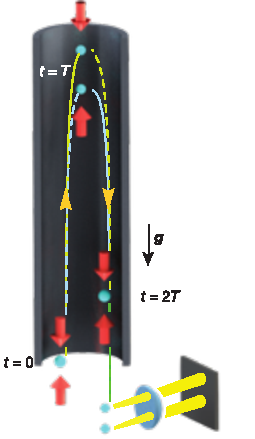
\includegraphics[height=6cm]{images/atomic_fountain.pdf}
  \end{textblock}
  \begin{textblock}{13}(1.0,2.25)
    \hfill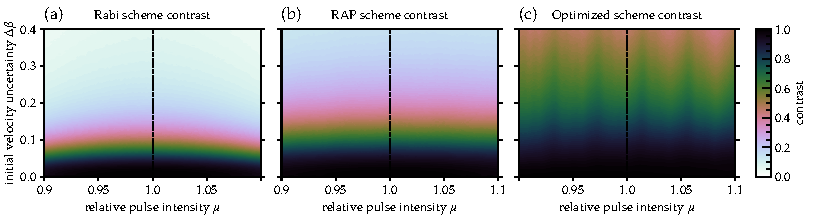
\includegraphics[trim=0 0 9.2cm 0,clip]{images/afioct/fig4.pdf}
  \end{textblock}
  \begin{textblock}{1}(14.0,2.25)
    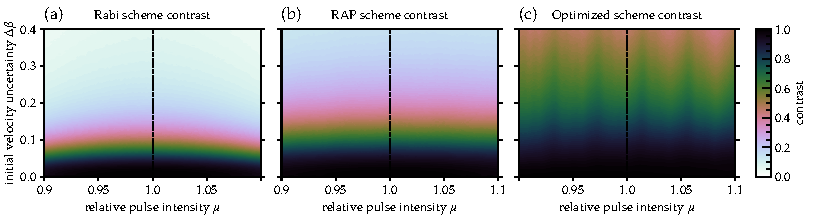
\includegraphics[trim=12.6cm 0 0 0,clip]{images/afioct/fig4.pdf} % colorbar
  \end{textblock}
  \begin{textblock}{10}(5.0,7.5)
    \onslide<1->{%
      \hfill\footnotesize{--- Goerz, Kasevich, Malinovsky.  Atoms 11, 36 (2023)}
    }
  \end{textblock}
\end{frame}

\begin{frame}{Atomic Fountain Interferometer -- Rapid Adiabatic Passage (RAP)}
  \begin{textblock}{3}(1.0,1.5)
    \includegraphics<1-2>[height=6cm]{images/atomic_fountain.pdf}
  \end{textblock}
  \begin{textblock}{3}(12.2,5.2)
    \includegraphics<2->[trim=9.0cm 0 0 0,clip,height=3cm]{images/afioct/fig1.pdf}
  \end{textblock}
  \begin{textblock}{14}(1.0,1.5)
    \hfill\includegraphics<1-2>[trim=8.3cm 0 0 0,clip]{images/afioct/fig2.pdf}
  \end{textblock}
  \begin{textblock}{14}(1.0,1.5)
    \hfill\includegraphics<3>[trim=6.0cm 0 0 0,clip]{images/afioct/fig3.pdf}
  \end{textblock}
  \begin{textblock}{10}(5.0,7.5)
    \footnotesize{--- Goerz, Kasevich, Malinovsky.  Atoms 11, 36 (2023)}
  \end{textblock}
\end{frame}


\begin{frame}{Atomic Fountain Interferometer -- Robustness RAP}
  \begin{textblock}{3}(1.0,1.5)
    \includegraphics<1-2>[height=6cm]{images/atomic_fountain.pdf}
  \end{textblock}
  \begin{textblock}{13}(1.0,2.25)
    \hfill\includegraphics<1>[trim=0 0 9.2cm 0,clip]{images/afioct/fig4.pdf}
  \end{textblock}
  \begin{textblock}{13}(1.0,2.25)
    \hfill\includegraphics<2>[trim=0 0 5.2cm 0,clip]{images/afioct/fig4.pdf}
  \end{textblock}
  \begin{textblock}{1}(14.0,2.25)
    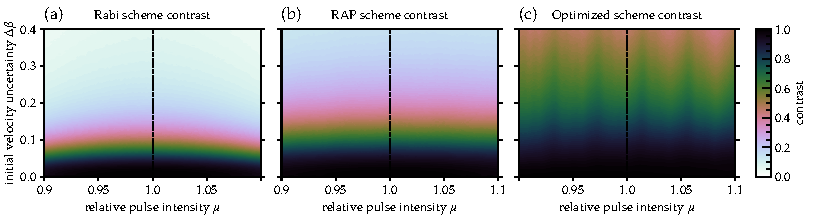
\includegraphics[trim=12.6cm 0 0 0,clip]{images/afioct/fig4.pdf} % colorbar
  \end{textblock}
  \begin{textblock}{10}(5.0,7.5)
    \onslide<1->{%
      \hfill\footnotesize{--- Goerz, Kasevich, Malinovsky.  Atoms 11, 36 (2023)}
    }
  \end{textblock}
\end{frame}

\begin{frame}{Atomic Fountain Interferometer -- Optimal Control (OCT)}
  \begin{textblock}{14}(1.0,1.5)
    \hfill\includegraphics<1>[trim=6.0cm 0 0 0,clip]{images/afioct/fig3.pdf}
  \end{textblock}
  \begin{textblock}{14}(1.0,2.0)
    \includegraphics<2>[trim=0 0 9.5cm 0, clip]{images/afioct/fig6.pdf}
  \end{textblock}
  \begin{textblock}{14}(1.0,2.0)
    \includegraphics<3>[trim=0 0 4.25cm 0, clip]{images/afioct/fig6.pdf}
  \end{textblock}
  \begin{textblock}{14}(1.0,2.0)
    \includegraphics<4>{images/afioct/fig6.pdf}
  \end{textblock}
  \begin{textblock}{14}(1.0,1.5)
    \hfill\includegraphics<5>[trim=6.0cm 0 0 0,clip]{images/afioct/fig3.pdf}
  \end{textblock}
  \begin{textblock}{14}(1.0,1.5)
    \hfill\includegraphics<6>[trim=0 0 0 0,clip]{images/afioct/fig7.pdf}
  \end{textblock}
  \begin{textblock}{10}(5.0,7.5)
    \onslide<1->{%
      \hfill\footnotesize{--- Goerz, Kasevich, Malinovsky.  Atoms 11, 36 (2023)}
    }
  \end{textblock}
\end{frame}


\begin{frame}{Atomic Fountain Interferometer -- Robustness OCT}
  \begin{textblock}{3}(1.0,1.5)
    \includegraphics<1>[height=6cm]{images/atomic_fountain.pdf}
  \end{textblock}
  \begin{textblock}{13}(1.0,2.25)
    \hfill\includegraphics<1>[trim=0 0 5.2cm 0,clip]{images/afioct/fig4.pdf}
  \end{textblock}
  \begin{textblock}{13}(1.0,2.25)
    \hfill\includegraphics<2>[trim=0 0 1.2cm 0,clip]{images/afioct/fig4.pdf}
  \end{textblock}
  \begin{textblock}{1}(14.0,2.25)
    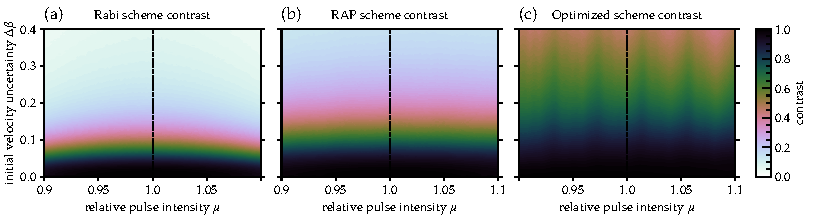
\includegraphics[trim=12.6cm 0 0 0,clip]{images/afioct/fig4.pdf}
  \end{textblock}
  \begin{textblock}{10}(5.0,7.5)
    \onslide<1->{%
      \hfill\footnotesize{--- Goerz, Kasevich, Malinovsky.  Atoms 11, 36 (2023)}
    }
  \end{textblock}
\end{frame}


\begin{frame}{JuliaQuantumControl}
  \begin{textblock}{15.5}(0.25,1.00)
    \includegraphics<2>[width=\textwidth]{images/JuliaQuantumControl}
    % \includegraphics<3>[width=\textwidth]{images/JuliaQuantumControlPackages}
  \end{textblock}
\end{frame}


\begin{frame}
  \begin{center}
    {\Large \color{DarkRed} \bf Why Julia?}
    \vspace{1.5cm}
    \pause
    \begin{itemize}
      \item Performance \pause -- compiles to low-level machine code (matches Fortran) \pause
      \item Flexibility \pause -- multiple dispatch\pause, ecosystem\pause
      \item Expressiveness \pause -- clean syntax, unicode, notebook environment
    \end{itemize}
  \end{center}
\end{frame}


\begin{frame}{JuliaQuantumControl}
  \begin{textblock}{15.5}(0.25,1.00)
    \includegraphics<1->[width=\textwidth]{images/JuliaQuantumControl.png}
  \end{textblock}
  \begin{textblock}{14.5}(0.75,5.28)
    \onslide<2>{%
      \begin{block}{Design Principle}
        \begin{center}
          Maximum performance and composability through abstract interfaces
        \end{center}
      \end{block}
    }
  \end{textblock}
\end{frame}

\begin{frame}{Optimization Functional}
  \begin{textblock}{15.5}(0.25,1.00)
    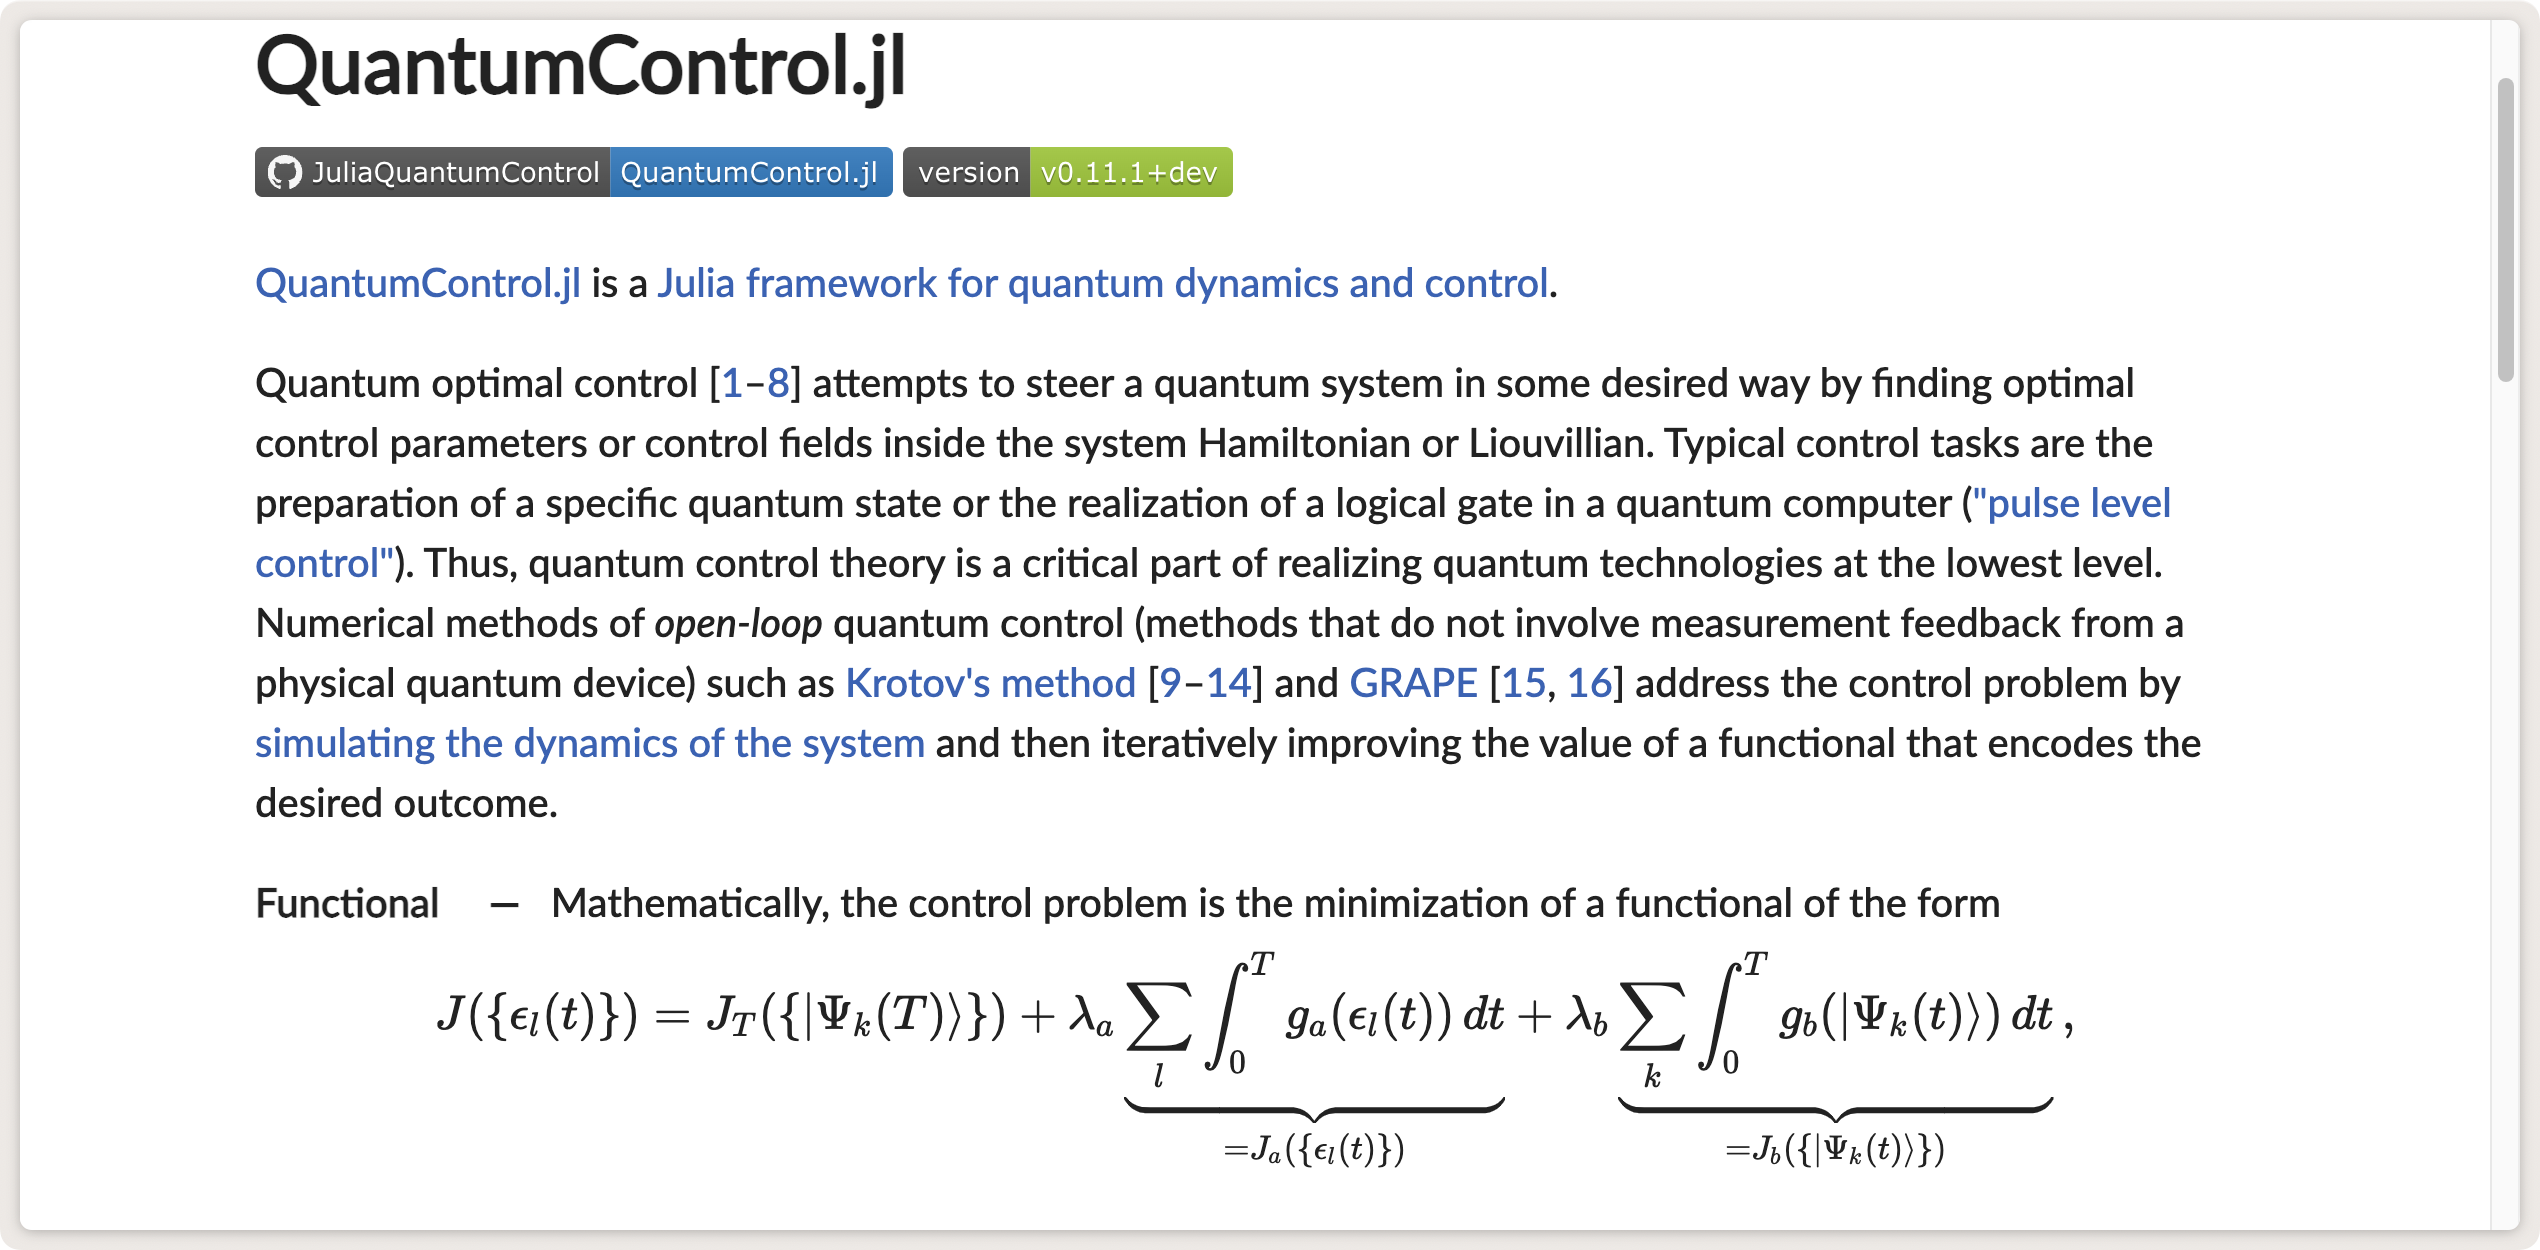
\includegraphics[width=\textwidth]{images/functional.png}
  \end{textblock}
\end{frame}

\begin{frame}{Control Problem and Trajectories}
  \begin{textblock}{15.5}(0.25,1.00)
    \includegraphics<1>[width=\textwidth]{images/api_controlproblem.png}
    \includegraphics<2>[width=\textwidth]{images/api_controlproblem2.png}
    \includegraphics<3>[width=\textwidth]{images/api_trajectory.png}
    \includegraphics<4>[width=\textwidth]{images/api_trajectory2.png}
  \end{textblock}
\end{frame}

\begin{frame}{Dynamical Generators}
  \begin{textblock}{15.5}(0.25,1.00)
    \includegraphics<1>[width=\textwidth]{images/glossary_generator.png}
    \includegraphics<2>[width=\textwidth]{images/api_check_generator.png}
  \end{textblock}
\end{frame}

\begin{frame}{Optimization schemes}
  \begin{textblock}{15.5}(0.25,1.50)
    \includegraphics<2>[width=\textwidth]{images/schemes_comparison.pdf}
  \end{textblock}
  \begin{textblock}{10}(5.0,7.2)
    \onslide<2>{%
      \hfill\footnotesize{--- Goerz, Carrasco, Malinovsky.  Quantum 6, 871 (2022)}
    }
  \end{textblock}
\end{frame}


\begin{frame}{Propagators}
  \begin{textblock}{15.5}(0.25,1.00)
    \includegraphics<2>[width=\textwidth]{images/api_propagator.png}
    \includegraphics<3>[width=\textwidth]{images/api_propagator2.png}
    \includegraphics<4>[width=\textwidth]{images/differentialequations.png}
  \end{textblock}
\end{frame}


\begin{frame}{Rotating Tractor Interferometer}
  \begin{textblock}{13.5}(1.25,0.75)
    \begin{center}
      \includegraphics<2>{images/pinwheel}
    \end{center}
  \end{textblock}
  \begin{textblock}{15.5}(1.5,1.50)
    \only<3->{%
      \includegraphics{images/rottai_concept}
    }
  \end{textblock}
  \begin{textblock}{8.0}(6.5,1.75)
    \only<4->{%
      \begin{equation*}
        H_{\pm}(\theta, t) = -\frac{\hbar^2}{2M}\frac{\partial^2}{\partial \theta^2} + V_0 \cos\left(m (\theta + \phi_{\pm}(t) )\right)
      \end{equation*}
    }
  \end{textblock}
  \begin{textblock}{14.0}(1.0,6.25)
    \only<4->{%
      In co-moving frame:
      \vspace{-1.1cm}
      \begin{equation*}
          \hspace{2.5cm}
          \tilde{H}_{\pm} (t)= -\frac{\hbar^2}{2M}\frac{\partial^2}{\partial \theta^2} + V_0 \cos\left(m \theta\right) - i \hbar \omega_{\pm}(t) \frac{\partial}{\partial \theta}
      \end{equation*}
    }
  \end{textblock}
  \begin{textblock}{10}(5.0,8.2)
    \onslide<2->{%
      \hfill\footnotesize{--- Dash, Goerz \emph{et al.} AVS Quantum Sci. 6, 014407 (2023)}
    }
  \end{textblock}
\end{frame}


\begin{frame}{Project-Specific Data Structures}
  \begin{textblock}{15.5}(0.25,1.00)
    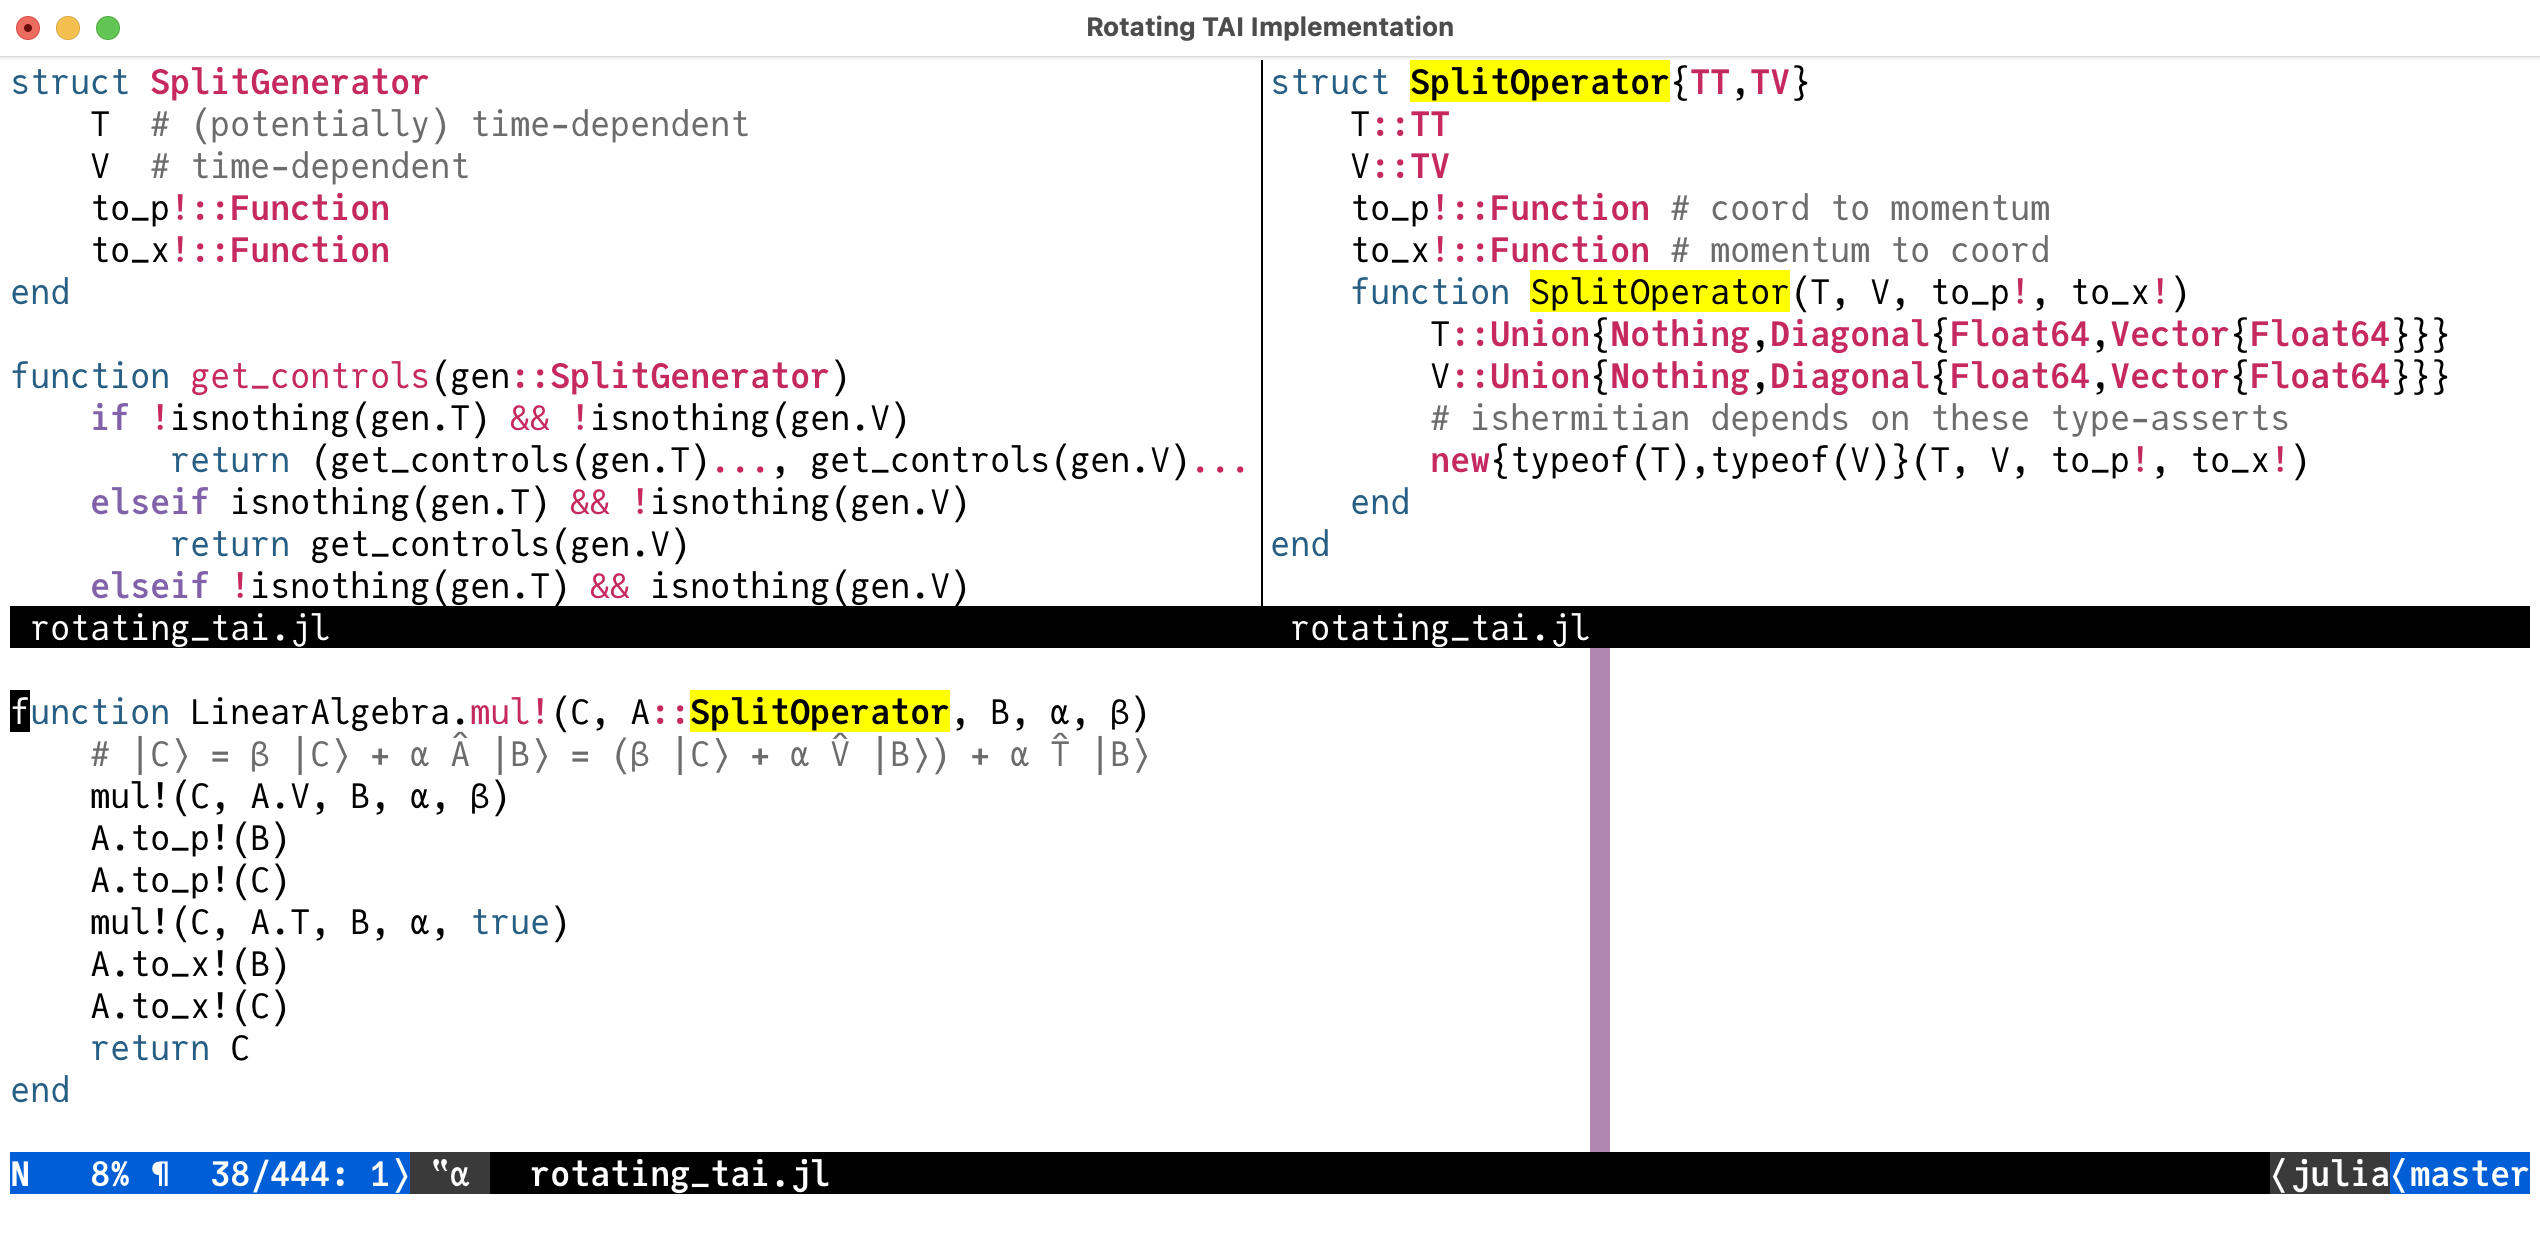
\includegraphics[width=\textwidth]{images/rottai_code}
  \end{textblock}
\end{frame}

\begin{frame}{Adiabatic Dynamics of Rotating TAI}
  \begin{textblock}{7.0}(0.5,1.00)
    \includegraphics<1-3>{images/animate_rottai/frame_000.pdf}
    \includegraphics<4>{images/animate_rottai/frame_100.pdf}
    \includegraphics<5>{images/animate_rottai/frame_200.pdf}
    \includegraphics<6->{images/animate_rottai/frame_300.pdf}
  \end{textblock}
  \begin{textblock}{7.0}(0.5,2.00)
    \onslide<2>{%
      \begin{center}
        {\color{DarkRed}$\pi/2$ pulse}
      \end{center}
    }
  \end{textblock}
  \begin{textblock}{7.0}(0.5,2.00)
    \onslide<9>{%
      \begin{center}
        {\color{DarkRed}inverse \\ $\pi/2$ pulse}
      \end{center}
    }
  \end{textblock}
  \begin{textblock}{7.0}(0.5,5.50)
    \onslide<3->{%
      \begin{equation*}
        \omega(t) = \begin{cases}
          \omega_{0} \sin^2\left(\frac{\pi t}{2 t_r}\right)         & 0 \leq t < t_r            \\
          \omega_{0}                                                & t_r \leq t < t_r + t_{\text{loop}}  \\
          \omega_{0} \cos^2\left(\frac{\pi t^\prime }{2t_r} \right) & T - t_r \leq t \leq T
        \end{cases}
      \end{equation*}
    }
  \end{textblock}
  \begin{textblock}{7.75}(8.0,2.00)
    \begin{center}
      \includegraphics<3-7>{images/adiabatic_dynamics_50πps_1}
      \includegraphics<8->{images/adiabatic_dynamics_50πps_2}
    \end{center}
  \end{textblock}
  \begin{textblock}{10}(5.0,8.2)
    \onslide<1->{%
      \hfill\footnotesize{--- Dash, Goerz \emph{et al.} AVS Quantum Sci. 6, 014407 (2023)}
    }
  \end{textblock}
\end{frame}

\begin{frame}{Interferometric Response of Rotating TAI}
  \begin{textblock}{15.5}(0.25,1.30)
    \begin{equation*}
      \Delta \Phi_S = \frac{4 m\Omega A}{\hbar}\,,
      \quad
      A
      = \frac{R^2}{2}
        \underbrace{\int_{0}^{T}\omega(t^\prime)dt^\prime}_{=\only<1-4>{n}\only<5>{2}\only<6>{10}\pi}
    \end{equation*}
  \end{textblock}
  \begin{textblock}{15.5}(0.25,3.00)
    \onslide<2->{%
      \begin{equation*}
        |c_{\pm}|^2
        = \frac{1}{2}
          \pm \frac{1}{2} \Re\left[{\color<3>{DarkRed}\eta} e^{-i \Delta\Phi}\right]
        \onslide<4->{%
          \qquad \rightarrow  \qquad
          |c_{-}|^2
          = \frac{1}{2} - \frac{\cos{\Delta\Phi}}{2} = \sin^2\left(\frac{\Delta\Phi}{2}\right)
        }
      \end{equation*}
    }
  \end{textblock}
  \begin{textblock}{4}(1.85,4.00)
    \onslide<3-4>{%
      \begin{equation*}
        \color{DarkRed}
        \eta = \braket{\Psi_{-}(\theta, T)|\Psi_{+}(\theta, T)}
        = 1 \quad \text{if adiabatic}
      \end{equation*}
    }
  \end{textblock}
  \begin{textblock}{15.5}(0.25,4.2)
    \onslide<5->{%
      \begin{center}
        \includegraphics<5>{images/cn_sim_results_1.pdf}
        \includegraphics<6>{images/cn_sim_results_2.pdf}
      \end{center}
    }
  \end{textblock}
  \begin{textblock}{10}(5.0,8.2)
    \onslide<5->{%
      \hfill\footnotesize{--- Dash, Goerz \emph{et al.} AVS Quantum Sci. 6, 014407 (2023)}
    }
  \end{textblock}
\end{frame}


\begin{frame}{Non-Adiabatic Dynamics of Rotating TAI}
  \begin{textblock}{7.75}(0.25,2.00)
    \includegraphics<1>{images/fidelity_map_1}
    \includegraphics<2-8>{images/fidelity_map_2}
  \end{textblock}
  \begin{textblock}{7.0}(8.5,2.25)
    \onslide<1-2>{%
      \begin{equation*}
        \omega(t) = \begin{cases}
          \omega_{0} \sin^2\left(\frac{\pi t}{2 t_r}\right)         & 0 \leq t < t_r            \\
          {\color{gray}\omega_{0}}                                  & {\color{gray}t_r \leq t < t_r + t_{\text{loop}}}  \\
          {\color{gray}\omega_{0} \cos^2\left(\frac{\pi t^\prime }{2t_r} \right)} & {\color{gray}T - t_r \leq t \leq T}
        \end{cases}
      \end{equation*}
      \vspace{2mm}
      \par
      $\ket{\Psi_{\text{tgt}}} = $ ground state of moving potential
    }
  \end{textblock}
  \begin{textblock}{7.75}(8.00,1.00)
    \includegraphics<3>{images/guess_dynamics_1.pdf}
    \includegraphics<4>{images/guess_dynamics_2.pdf}
    \includegraphics<5>{images/guess_dynamics_3.pdf}
    \includegraphics<6>{images/guess_dynamics_4.pdf}
    \includegraphics<7>{images/guess_dynamics_5.pdf}
    \includegraphics<8->{images/guess_dynamics_6.pdf}
  \end{textblock}
  \begin{textblock}{7.75}(0.25,2.00)
    \includegraphics<9-11>{images/guess_sagnac_1.pdf}
    \includegraphics<12>{images/guess_sagnac_2.pdf}
  \end{textblock}
  \begin{textblock}{7.75}(0.25,5.75)
    \onslide<9->{%
      \begin{equation*}
        \Delta \Phi_S = \frac{4 m\Omega A}{\hbar}\,,
        \quad
        A = \frac{R^2}{2} \cdot 10\pi
      \end{equation*}
    }
  \end{textblock}
  \begin{textblock}{7.75}(0.25,7.00)
    \only<9>{%
      \begin{equation*}
        |c_{-}|^2
        = \frac{1}{2} - \frac{\cos{\Delta\Phi}}{2} = \sin^2\left(\frac{\Delta\Phi}{2}\right)
      \end{equation*}
    }
    \only<10->{%
      \begin{equation*}
        |c_{-}|^2
        = \frac{1}{2} - \frac{1}{2} \Re\left[{\color<11>{DarkRed}\eta} e^{-i \Delta\Phi}\right]
      \end{equation*}
    }
  \end{textblock}
  \begin{textblock}{10}(5.0,8.2)
    \onslide<1-6>{%
      \hfill\footnotesize{--- Dash, Goerz \emph{et al.} AVS Quantum Sci. 6, 014407 (2023)}
    }
  \end{textblock}
\end{frame}


\begin{frame}{Rotating TAI Control Problem}
  \begin{textblock}{15.0}(0.5,1.20)
    \begin{center}
      \begin{equation*}
        \omega(t) = \begin{cases}
          \omega_{\text{opt}}(t)  & 0 \leq t < t_r            \\
          \omega_{0}              & t_r \leq t < t_r + t_{\text{loop}}  \\
          \omega_{\text{opt}}(t') & T - t_r \leq t \leq T
        \end{cases}
      \end{equation*}
      \par
      \vspace{8mm}
      Find $\omega_{\text{opt}}(t)$ for short $t_r$ so that
      \begin{equation*}
        \color{DarkRed}
        \Psi(\theta, t=0) \rightarrow \Psi_{\text{tgt}}(\theta, t=t_r)
      \end{equation*}
      where $\ket{\Psi_{\text{tgt}}} = $ ground state of moving potential
    \end{center}
  \end{textblock}
\end{frame}


\begin{frame}{Optimization with QuantumControl.jl}
  \begin{textblock}{15.5}(0.25,1.00)
    \includegraphics<1-2>[width=\textwidth]{images/optimization_screenshot1}
    \includegraphics<3>[width=\textwidth]{images/optimization_screenshot2}
  \end{textblock}
  \begin{textblock}{12.8}(2.0,3.70)
    \onslide<2>{%
      \begin{block}{Guided Control}
        \vspace{2mm}
        \begin{equation*}
          \omega_{\text{opt}}(t) = \omega(t) + S(t)\delta\omega(t)
        \end{equation*}
        \vspace{2mm}
      \end{block}
    }
  \end{textblock}
\end{frame}


\begin{frame}{Optimized Dynamics or Rotating TAI}
  \begin{textblock}{7.75}(0.25,1.00)
    \includegraphics<1-6>{images/guess_dynamics.pdf}
  \end{textblock}
  \begin{textblock}{7.75}(8.00,1.00)
    \includegraphics<2>{images/opt_dynamics_1.pdf}
    \includegraphics<3>{images/opt_dynamics_2.pdf}
    \includegraphics<4>{images/opt_dynamics_3.pdf}
    \includegraphics<5>{images/opt_dynamics_5.pdf}
    \includegraphics<6->{images/opt_dynamics_6.pdf}
  \end{textblock}
  \begin{textblock}{7.75}(0.25,2.00)
   \includegraphics<7>{images/opt_sagnac_1.pdf}
   \includegraphics<8->{images/opt_sagnac_2.pdf}
  \end{textblock}
  \begin{textblock}{7.75}(0.25,5.75)
    \onslide<7->{%
      \begin{equation*}
        \Delta \Phi_S = \frac{4 m\Omega A}{\hbar}\,,
        \quad
        A = \frac{R^2}{2} \cdot 10\pi
      \end{equation*}
    }
  \end{textblock}
  \begin{textblock}{7.75}(0.25,7.00)
   \only<7>{%
     \begin{equation*}
       |c_{-}|^2
       = \frac{1}{2} - \frac{1}{2} \Re\left[\eta e^{-i \Delta\Phi}\right]
     \end{equation*}
   }
   \only<8->{%
     \begin{equation*}
       |c_{-}|^2
       = \frac{1}{2} - \frac{\cos{\Delta\Phi}}{2} = \sin^2\left(\frac{\Delta\Phi}{2}\right)
     \end{equation*}
   }
  \end{textblock}
\end{frame}


\begin{frame}{Nuclear Spin Gyroscope}
  \begin{textblock}{15}(0.5,1.0)
    \onslide<2>{%
      \begin{center}
        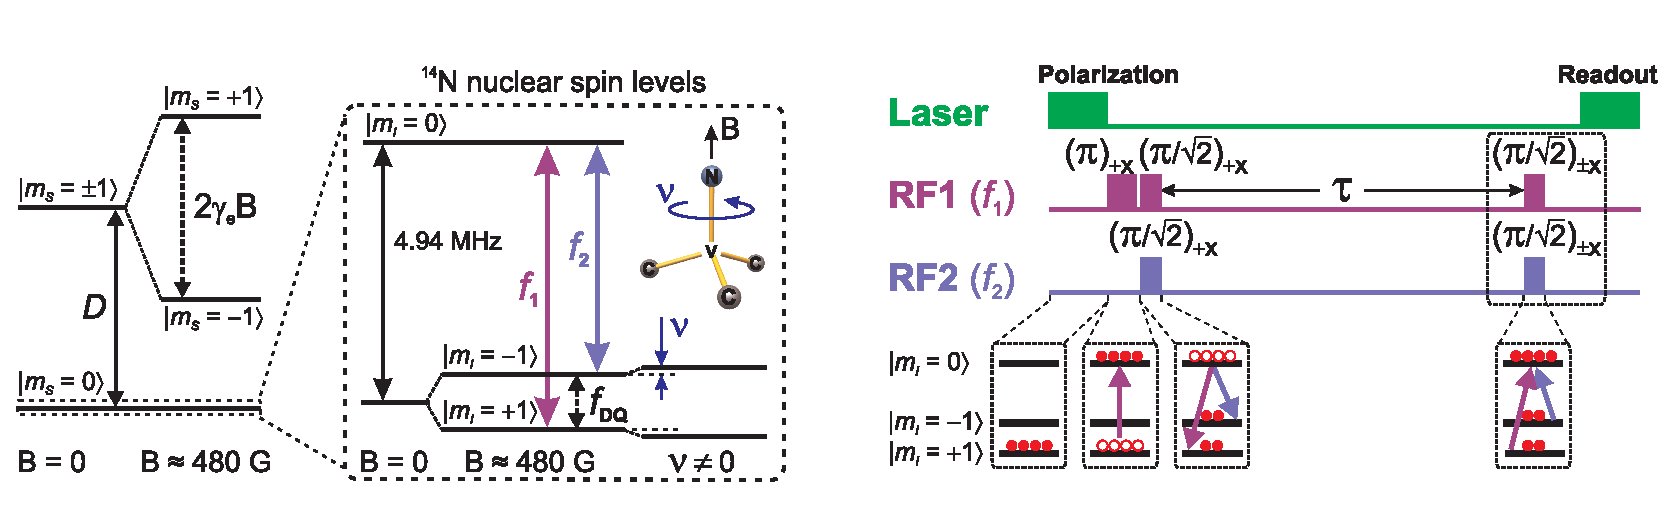
\includegraphics[width=\textwidth]{images/JarmolaSA2021_Fig2}
      \end{center}
      \hfill {\footnotesize --- Adapted from Fig 2 of Jarmola \textit{et. al.} Sci. Adv. 7, eabl3840 (2021)}
    }
  \end{textblock}
\end{frame}


\begin{frame}{NV Center Hamiltonian with Crosstalk}
  \begin{textblock}{6}(0.5,2.00)
    %\documentclass[aps, pra, onecolumn, superscriptaddress, floatfix]{revtex4-2}
%\usepackage[utf8]{inputenc}
%\usepackage{amsmath}
%\usepackage{mathpazo}
%\usepackage{braket}
%\usepackage[hidelinks]{hyperref}
%\usepackage{graphicx}
%
%
%\usepackage{tikz,pgflibraryshapes}
%\usetikzlibrary{calc}
%\usetikzlibrary{decorations.pathmorphing}
%\usetikzlibrary{arrows.meta}
%\usetikzlibrary{positioning}
%
%\usepackage[psfixbb,graphics,tightpage,active]{preview}
%
%\PreviewEnvironment{tikzpicture}
%
\tikzset{arrow/.style={-{Latex[length=3pt]}}}
\tikzset{doublearrow/.style={{Latex[length=3pt]}-{Latex[length=3pt]}}}
%
%\begin{document}
\begin{tikzpicture}
  \definecolor{red}{RGB}{192,0,0}
  \definecolor{blue}{RGB}{3,110,189}
  \footnotesize
  % \node[right] at (-0.7, 3.5)  {(a)};
  % \node[right] at (3.2, 3.5)  {(b)};
  % \begin{scope}[xscale=0.25,yscale=0.28] % Level Diagram
  \begin{scope}[xscale=0.4,yscale=0.4] % Level Diagram
    \def\LevelMinusOne{3}
    \def\LevelZero{10}
    \def\DeltaP{2}
    \def\DeltaS{4}
    \def\Width{10}
    \def\xOmegaOne{0.05}  % x coordinate for ω₁ line, as portion of \Width
    \def\xOmegaP{0.275}  % x coordinate for ωₚ line, as portion of \Width
    \def\xOmegaS{0.725}  % x coordinate for ωₛ line, as portion of \Width
    \pgfmathsetmacro{\SinglePhotonDetuning}{0.5*(\DeltaP + \DeltaS)}
    % Energy Levels
    \draw[thick] (0, 0) node[left]{$\ket{+1}$} -- +(\Width, 0);
    \draw[thick] (0.4*\Width, \LevelMinusOne) -- ++(0.6*\Width, 0) node[right]{$\ket{-1}$};
    \draw[thick] (0, \LevelZero) node[left]{$\ket{0}$} -- +(\Width, 0);
    % Detuning Levels
    \draw[dashed] (0.15 * \Width, \LevelZero - \DeltaP) -- +(0.35 * \Width, 0);
    \draw[dashed] (0.35 * \Width, \LevelZero - \DeltaS) -- +(0.5 * \Width, 0);
    \draw[dashed] (0.475 * \Width, \LevelZero - \SinglePhotonDetuning) -- +(0.2 * \Width, 0);
    %  Arrows
    \draw[arrow, red, thick] (\xOmegaP * \Width, 0) -- +(0, \LevelZero - \DeltaP) node[midway, left, red]{$\omega_p$};
    \draw[arrow] (\xOmegaOne * \Width, 0) -- +(0, \LevelZero) node[midway, left]{$\omega_1$};
    \draw[arrow] (\xOmegaP * \Width, \LevelZero) -- +(0, -\DeltaP) node[midway, left]{$\Delta_p$};
    \draw[arrow, blue, thick] (\xOmegaS * \Width, \LevelMinusOne) -- +(0, \LevelZero - \DeltaS - \LevelMinusOne) node[midway, right, blue]{$\omega_s$};
    \draw[arrow] (\xOmegaS * \Width, \LevelZero) -- +(0, -\DeltaS) node[midway, right]{$\Delta_s$};
    \draw[arrow] (0.95 * \Width, \LevelMinusOne) -- +(0, \LevelZero - \LevelMinusOne) node[midway, right]{$\omega_2$};
    \draw[arrow] (0.425 * \Width, \LevelZero - \DeltaS) -- +(0, \DeltaS - \DeltaP) node[midway, left]{$\delta$};
    \draw[arrow] (0.575 * \Width, \LevelZero) -- +(0, -0.5 * \DeltaS - 0.5 * \DeltaP) node[pos=0.28, left]{$\Delta$};
    \draw[arrow] (0.575 * \Width, 0) -- +(0, \LevelMinusOne) node[midway, right]{$\omega_{12}$};
  \end{scope}
  %\begin{scope}[xscale=0.7, yscale=1.0, xshift=5.5cm, yshift=0.55cm] % pulse sequence
  %  \def\pulseLength{1.5}
  %  \def\tauLength{1.5}
  %  \def\extraBeforeAfter{0.5}
  %  \def\boxPad{0.2}
  %  \pgfmathsetmacro{\timeLength}{2*\extraBeforeAfter + 2*\pulseLength + \tauLength}
  %  \draw[blue, thick] (-\extraBeforeAfter, 0) -- +(\timeLength, 0);
  %  \draw[red, thick] (-\extraBeforeAfter, 1) -- +(\timeLength, 0);
  %  \draw[dashed] (0,-0.5) node[below]{0} -- +(0, 3);
  %  \draw[dashed] (\pulseLength,-0.5) node[below]{$T$} -- +(0, 3);
  %  \draw[dashed] (\pulseLength + \tauLength, -0.5) node[below]{$T+\tau$} -- +(0, 3);
  %  \draw[dashed] (2 * \pulseLength + \tauLength,-0.5) node[below]{$2T + \tau$} -- +(0, 3);
  %  \draw[fill=blue] (\boxPad, 0) rectangle +(\pulseLength - 2 * \boxPad, 1-\boxPad) node[pos=.5,white] {$\Omega_s$};;
  %  \draw[fill=blue] (\pulseLength + \tauLength + \boxPad, 0) rectangle +(\pulseLength - 2 * \boxPad, 1-\boxPad) node[pos=.5,white] {$\Omega_s$};;
  %  \draw[fill=red] (\boxPad, 1) rectangle +(\pulseLength - 2 * \boxPad, 1-\boxPad) node[pos=.5,white] {$\Omega_p$};;
  %  \draw[fill=red] (\pulseLength + \tauLength + \boxPad, 1) rectangle +(\pulseLength - 2 * \boxPad, 1-\boxPad) node[pos=.5,white] {$\Omega_p$};;
  %  \draw[semithick, rounded corners] (0, -\boxPad) rectangle +(\pulseLength, 2 + \boxPad);
  %  \draw[semithick, rounded corners] (\pulseLength + \tauLength, -\boxPad) rectangle +(\pulseLength, 2 + \boxPad);
  %  \node at (0.5 * \pulseLength, 2.25) {$\pi/2$};
  %  \node at (\pulseLength + \tauLength + 0.5 * \pulseLength, 2.25) {$\pi/2$};
  %  \draw[doublearrow] (\pulseLength, 2.25) -- +(\tauLength, 0) node[midway, below]{$\tau$};
  %\end{scope}
\end{tikzpicture}
%\end{document}

    % \includegraphics<1>[trim=0 0 4cm 5mm,clip]{images/nvcenter_system_diagram.pdf}
  \end{textblock}
  \begin{textblock}{8}(7.0,2.00)
    \only<1>{%
      \begin{equation*}
        \Op{H} = \begin{pmatrix}
              0     & \Omega(t) &    0                       \\
          \Omega(t) & \omega_1  & \Omega(t)                  \\
              0     & \Omega(t)  & \omega_1 - \omega_2
        \end{pmatrix}
      \end{equation*}
      \begin{align*}
          \Omega(t) &= \Omega_p(t) \cos\left(\omega_p t + \phi_p(t) + \phi_p^{(i)}\right)  \\
                    &\quad + \Omega_s(t) \cos\left(\omega_s t + \phi_s(t) + \phi_s^{(i)}\right)
      \end{align*}
    }
    \only<2>{%
      \begin{equation*}
        \Op{H}_{\text{RWA}} = \begin{pmatrix}
            -\frac{\delta}{2}  &   \Omega_{1,0}(t)   &    0              \\
            \Omega_{1,0}^*(t)  &      \Delta         & \Omega_{0,-1}(t)  \\
                    0          & \Omega_{0,-1}^*(t)  & \frac{\delta}{2}
        \end{pmatrix}
      \end{equation*}
      \begin{align*}
        \Omega_{1,0}(t) &= \frac{\Omega_p(t)}{2} e^{i \phi_p^{(i)}} + \frac{\Omega_s(t)}{2} e^{i\phi_s^{(i)}} e^{-i \omega_{ps} t} \\
        \Omega_{0,-1}(t) &= \frac{\Omega_s^*(t)}{2} e^{-i \phi_p^{(i)}} + \frac{\Omega_p^*(t)}{2} e^{-i\phi_s^{(i)}} e^{-i \omega_{ps} t}
      \end{align*}
    }
  \end{textblock}
  \begin{textblock}{15.5}(0.25,1.00)
    \includegraphics<3>[width=\textwidth]{images/ramsey_ham_code.png}
  \end{textblock}
\end{frame}


\begin{frame}{Parameterized Pulses}
  \begin{textblock}{15.5}(0.25,1.00)
    \includegraphics<2>[width=\textwidth]{images/nvramsey_nb_parameterziation.png}
    \includegraphics<3>[width=\textwidth]{images/pulse_parameterization.png}
  \end{textblock}
\end{frame}


\begin{frame}{Population Response Signal}
  \begin{textblock}{15}(0.5,1.0)
    \begin{center}
      \includegraphics<2>{images/ramsey_1}
      \includegraphics<3>{images/ramsey_2}
      \includegraphics<4>{images/ramsey_3}
      \includegraphics<5->{images/ramsey_4}
    \end{center}
  \end{textblock}
  \begin{textblock}{15}(0.5,5.0)
    \begin{center}
      \includegraphics<2-5>[height=3.5cm]{images/JarmolaSA2021_Fig2}
    \end{center}
  \end{textblock}
  \begin{textblock}{13}(1.5,5.5)
    \onslide<6->{%
      \begin{center}
        \begin{block}{}
          \begin{equation*}
            J_T(\{\ket{\Psi_{\mu,\tau}(T)}\})
            = \sum_{\mu} \left\vert
            \text{FFT}([P_0({\color<7>{DarkRed}\tau}; {\color<7>{DarkRed}\mu})]) - \text{FFT}([P_0({\tau}; {\mu}=1)])
              \right\vert
          \end{equation*}
          Make spectrum for any $\mu$ look like spectrum for $\mu = 1$
        \end{block}
      \end{center}
    }
  \end{textblock}
\end{frame}


\begin{frame}{NV Center Optimization Problem}
  \begin{textblock}{15.5}(0.25,1.00)
    \includegraphics<2,6>[width=\textwidth]{images/nvramsey_nb_problem.png}
    \includegraphics<1>[width=\textwidth]{images/nvramsey_nb_problem1.png}
    \includegraphics<3-4>[width=\textwidth]{images/nvramsey_nb_problem2.png}
    \includegraphics<5>[width=\textwidth]{images/nvramsey_nb_problem3.png}
    \includegraphics<7->[width=\textwidth]{images/nvramsey_nb_problem4.png}
  \end{textblock}
  \begin{textblock}{13}(1.5,5.5)
    \onslide<1-3,5-6>{%
      \begin{center}
        \begin{block}{}
          \begin{equation*}
            J_T(\{\ket{\Psi_{\mu,\tau}(T)}\})
            = \sum_{\mu} \left\vert
            {\color<6>{DarkRed}\text{FFT}}([P_0({\color<1-5>{DarkRed}\tau}; {\color<1>{DarkRed}\mu})]) - {\color<6>{DarkRed}\text{FFT}}([P_0({\color<2-5>{DarkRed}\tau}; {\mu}=1)])
              \right\vert
          \end{equation*}
          Make spectrum for any $\mu$ look like spectrum for $\mu = 1$
        \end{block}
      \end{center}
    }
  \end{textblock}
  \begin{textblock}{13}(1.5,5.5)
    \onslide<4>{%
      \begin{center}
        \begin{block}{}
          \begin{equation*}
            \Omega_{1,0}(t) = \frac{\Omega_p(t)}{2} e^{i \color{DarkRed}\phi_p^{(i)}} + \frac{\Omega_s(t)}{2} e^{i \color{DarkRed}\phi_s^{(i)}} e^{-i \omega_{ps} t}
          \end{equation*}
          Absorb phase difference in RF pulse
        \end{block}
      \end{center}
    }
  \end{textblock}
  \begin{textblock}{13}(1.5,2.05)
    \onslide<7->{%
      \begin{center}
        \begin{block}{}
          \begin{equation*}
            J_T(\{\ket{\Psi_{\mu,\tau}(T)}\})
            = \sum_{\mu} \left\vert
            {\color{DarkRed}\text{FFT}}([P_0({\tau}; {\mu})]) - {\color{DarkRed}\text{FFT}}([P_0({\tau}; {\mu}=1)])
              \right\vert
          \end{equation*}
          Make spectrum for any $\mu$ look like spectrum for $\mu = 1$
        \end{block}
      \end{center}
    }
  \end{textblock}
\end{frame}

\begin{frame}{Semi-automatic differentiation}
  \begin{textblock}{13}(1.5,2.05)
    \onslide<1>{%
      \begin{center}
        \begin{block}{}
          \begin{equation*}
            J_T(\{\ket{\Psi_{\mu,\tau}(T)}\})
            = \sum_{\mu} \left\vert
            {\color{DarkRed}\text{FFT}}([P_0({\tau}; {\mu})]) - {\color{DarkRed}\text{FFT}}([P_0({\tau}; {\mu}=1)])
              \right\vert
          \end{equation*}
          Make spectrum for any $\mu$ look like spectrum for $\mu = 1$
        \end{block}
      \end{center}
    }
  \end{textblock}
  \begin{textblock}{7}(8.5,2.25)
    \onslide<3>{%
      Automatic Differentiation:\par
      evaluate $J_T$ inside AD framework
    }
  \end{textblock}
  \begin{textblock}{14}(1.0,4.0)
    \onslide<4,5>{%
      \begin{block}{Semi-AD}
        Use a chain rule to split the gradient into
        \begin{itemize}
          \item a numerically expensive but analytic part
          \item a non-analytic but computationally cheap part
      \end{itemize}
      \end{block}
    }
  \end{textblock}
  \begin{textblock}{7}(1.0,2.0)
    \onslide<2->{%
      \begin{equation*}
        \begin{split}
          \nabla J_T
          &= \frac{\partial J_T\only<5->{(\{\Psi_k(T)\})}}{\partial \epsilon_{nl}}
          \\
          \onslide<6->{%
          &= 2 \Re \Bigg[
            \sum_k
              {\color<6>{white}\underbrace{\color{black}\frac{\partial J_T}{\partial \ket{\Psi_k(T)}}}_{\equiv \bra{\chi_k}}}
              \frac{\partial \ket{\Psi_k(T)}}{\partial \epsilon_{nl}}
            \Bigg]
          }
          \\
          \onslide<8->{%
          &= 2 \Re \Bigg[
            \sum_k
              \frac{\partial}{\partial \epsilon_{nl}}
              {\braket{\chi_k(T) | \Psi_k(T)}}
            \Bigg]
          }
        \end{split}
      \end{equation*}
    }
  \end{textblock}
  \begin{textblock}{7}(8.5,2.5)
    \includegraphics<9->[width=\textwidth]{images/grape_scheme}
  \end{textblock}
  \begin{textblock}{15}(1.0,7.5)
    \onslide<4->{%
      \footnotesize{--- Goerz, Carrasco, Malinovsky.  Quantum 6, 871 (2022)}
    }
  \end{textblock}
\end{frame}


\begin{frame}{NV Center Optimized Pulses}
  \begin{textblock}{15.5}(0.25,1.00)
    \includegraphics<2>[width=\textwidth]{images/nvramsey_nb_solution1.png}
    \includegraphics<3>[width=\textwidth]{images/nvramsey_nb_solution2.png}
  \end{textblock}
\end{frame}


\begin{frame}{Optimized Signal Spectrum}
  \begin{textblock}{15}(0.5,1.0)
    \begin{center}
      \includegraphics<1>{images/ramsey_4}
      \includegraphics<2>{images/ramsey_5}
      \includegraphics<3>{images/ramsey_6}
      \includegraphics<4>{images/ramsey_7}
      \includegraphics<5>{images/ramsey_8}
    \end{center}
  \end{textblock}
  \begin{textblock}{13}(1.5,5.5)
    \onslide<1>{%
      \begin{center}
        \begin{block}{}
          \begin{equation*}
            J_T(\{\ket{\Psi_{\mu,\tau}(T)}\})
            = \sum_{\mu} \left\vert
                \text{FFT}([P_0(\tau; \mu)]) - \text{FFT}([P_0(\tau; \mu=1)])
              \right\vert
          \end{equation*}
          Make spectrum for any $\mu$ look like spectrum for $\mu = 1$
        \end{block}
      \end{center}
    }
  \end{textblock}
\end{frame}

\begin{frame}{Conclusion}
  \begin{textblock}{13}(1.5,1.5)
    \onslide<1->{%
      \begin{itemize}
        \item<2-> Quantum Interferometry Implementations
          \begin{itemize}
            \item<3-> Atomic Fountain Interferometer: robust momentum space transfer
            \item<4-> Rotating Tractor Interferometer: non-adiabatic phase space transport
            \item<5-> Nuclear Spin Gyroscope: ``double quantum'' control, spectral optimization
          \end{itemize}
      \end{itemize}
    }
  \end{textblock}
  \begin{textblock}{14}(1.0,3.75)
    \includegraphics<6>[width=\textwidth]{images/attribution.pdf}
  \end{textblock}
  \begin{textblock}{13}(1.5,4.0)
    \onslide<7->{%
      \begin{itemize}
        \item<7-> QuantumControl.jl Framework
          \begin{itemize}
            \item<8-> Define control problems in terms of ``trajectories''
            \item<9-> Define dynamics in terms of ``generators'' and stateful ``propagators''
            \item<10-> Separate ``control amplitudes`` from actual ``controls''
            \item<11-> Efficient project-specific data structures through multiple dispatch
          \end{itemize}
      \end{itemize}
    }
  \end{textblock}
  \begin{textblock}{13}(1.5,7.0)
    \onslide<12>{%
      \begin{center}
        {\color{DarkRed}
        \Large Thank You!
        }
      \end{center}
    }
  \end{textblock}
\end{frame}


%%%%%%%%%%%%%%%%%%%%%%%%%%%%%%%%%%%%%%%%%%%%%%%%%%%%%%%%%%%%
\appendix
\backupbegin

\begin{frame}\end{frame}

\begin{frame}{Semi-Automatic Differentiation}
  \begin{textblock}{14}(1.0,1.25)
    \only<1>{{\color{Red}\bf Quantum 6, 871 (2022) --- arXiv:2205.15044}}
  \end{textblock}
  \begin{textblock}{14}(1.0,1.75)
    \only<1>{%
      \frame{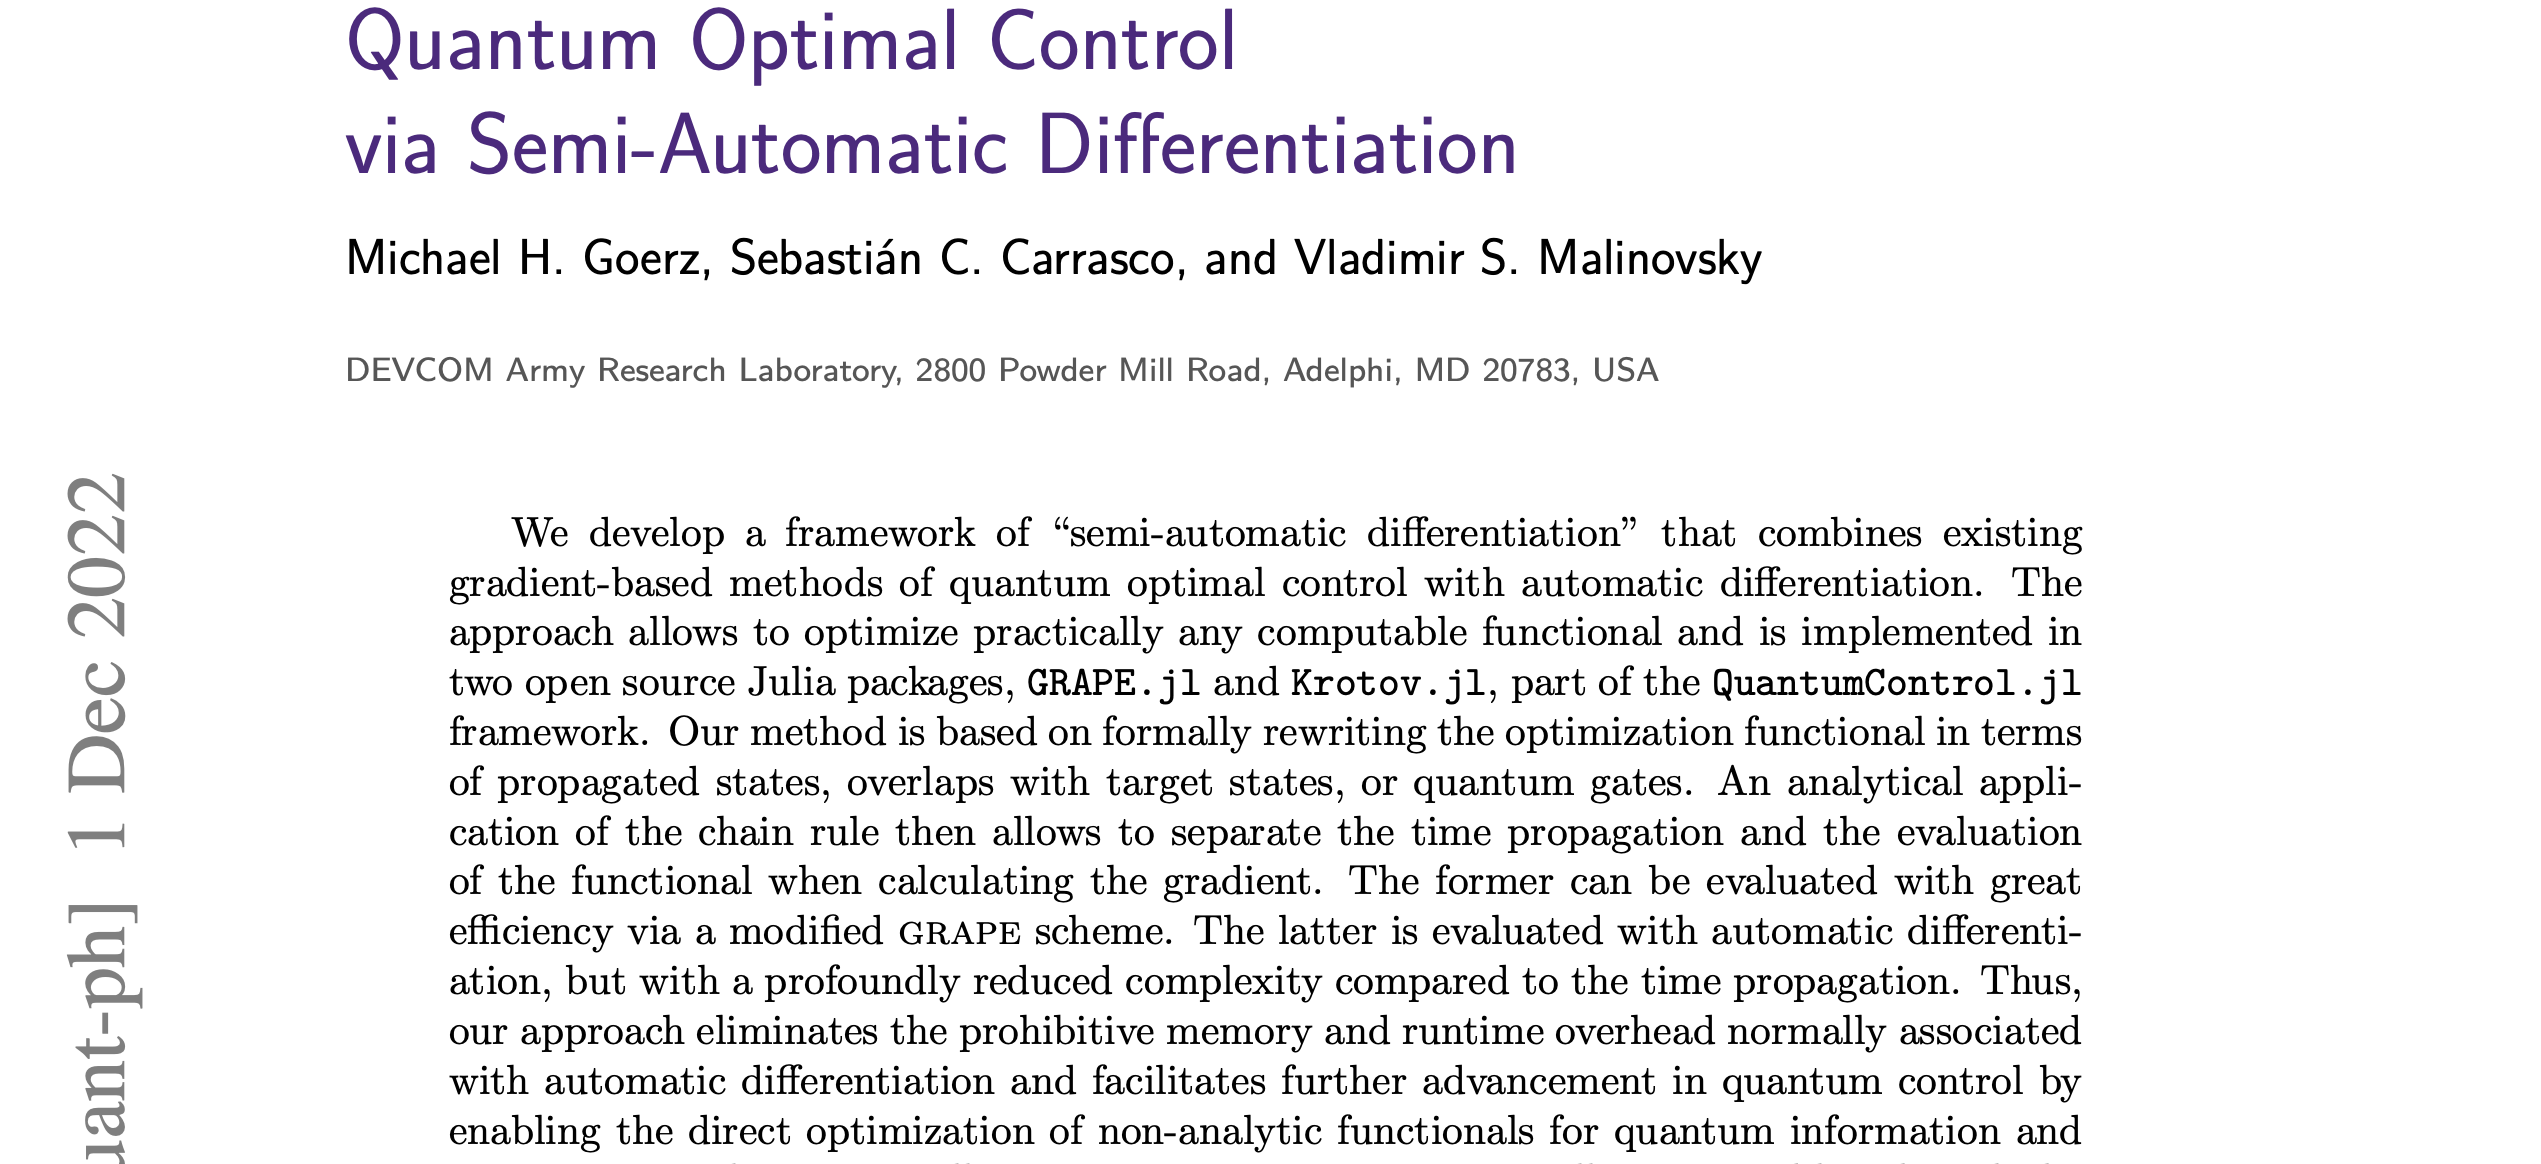
\includegraphics[width=\textwidth]{images/SemiAD_firstpage}}
    }
  \end{textblock}
  \begin{textblock}{14}(1.0,6.25)
    \only<4>{{\color{Red}\bf Goerz \emph{at al.} Quantum 6, 871 (2022) --- arXiv:2205.15044}}
  \end{textblock}
  \begin{textblock}{3.0}(12.25,1.75)
    \only<1>{%
      \begin{center}
        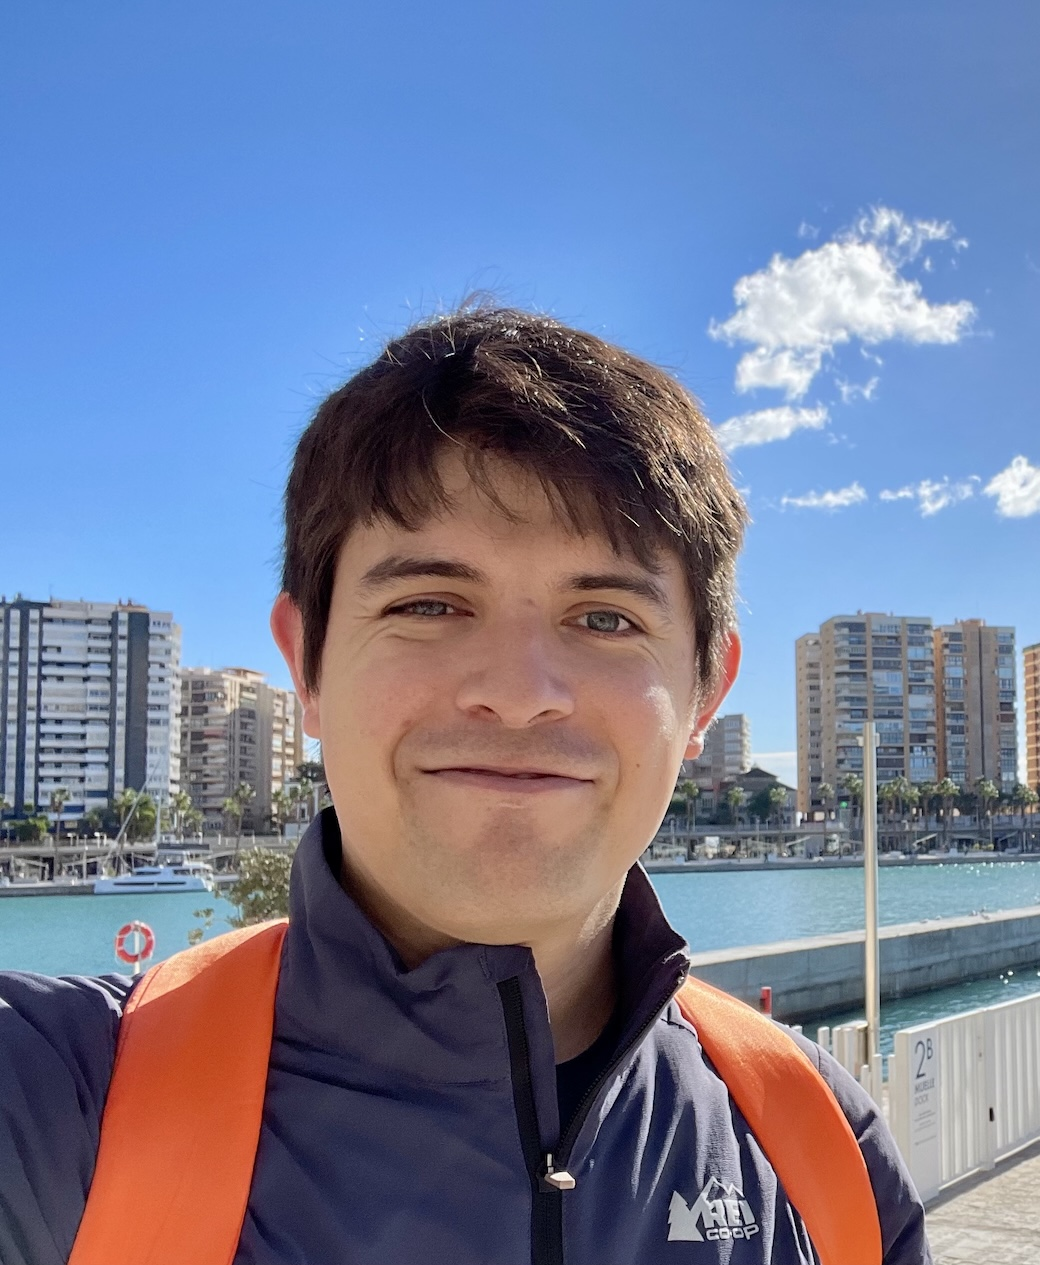
\includegraphics[width=1.5cm]{images/profile/seba.jpeg}\\
        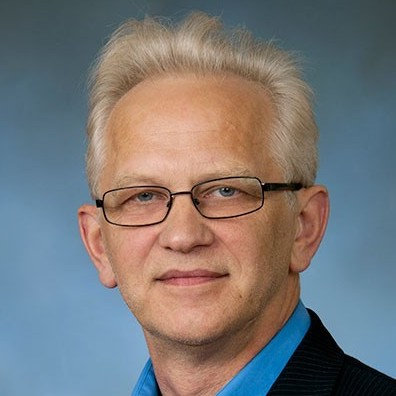
\includegraphics[width=1.5cm]{images/profile/vlad.jpg}
      \end{center}
    }
  \end{textblock}
  \begin{textblock}{10}(3.0, 7.02)
    \only<1>{\tiny
      \setbeamercolor{upcol}{fg=black,bg=gray!20}
      \setbeamercolor{lowcol}{fg=black,bg=gray!10}
      \begin{beamerboxesrounded}[upper=upcol,lower=lowcol]{Funding}
       DEVCOM Army Research Laboratory, Cooperative Agreement Numbers W911NF-16-2-0147, \\W911NF-21-2-0037; DIRA-TRC No. DTR19-CI-019
      \end{beamerboxesrounded}
    }
  \end{textblock}
  \begin{textblock}{15}(0.5, 1.0)
    \only<2->{%
      \begin{align*}
        \onslide<3->{\nabla}J(\{\epsilon_{nl}\})
          &= \onslide<3->{\frac{\partial}{\partial_{\epsilon_{nl}}}}
              J_T(\{\ket{\Psi_k(T)}\}) + \dots \\
        \onslide<5->{%
          &= 2\Re \sum_k
            \underbrace<6->{\frac{\partial J_T}{\partial \ket{\Psi_k(T)}}}_{%
              \equiv \bra{\chi_k(T)}
            }
            \frac{\partial \ket{\Psi_k(T)}}{\partial \epsilon_{nl}}
            \onslide<6->{%
              ; \qquad {\color<8->{DarkRed}\ket{\chi_k(T)} = \frac{\partial J_T}{\partial \bra{\Psi_k(T)}}}
            }
            \\
        }
        \onslide<7->{%
          &= 2 \Re \sum_k \frac{\partial}{\partial \epsilon_{nl}} \langle \chi_k(T) \vert \Psi_k(T) \rangle \\
        }
        \onslide<9->{%
          &= 2 \Re \sum_k \frac{\partial}{\partial \epsilon_{nl}} \langle \chi_k(T) \vert
              \Op{U}_N \dots \Op{U}_{n+1} \Op{U}_{n}  \Op{U}_{n-1} \dots \Op{U}_1  \vert
              \Psi_k(t=0) \rangle  \\
        }
        \onslide<10->{%
          &= 2 \Re \sum_k
            \underbrace<11->{%
              \Big\langle \chi_k(T) \Big\vert \Op{U}_N \dots \Op{U}_{n+1} {\color<12>{DarkRed}\frac{\partial \Op{U}_n}{\partial \epsilon_{nl}}}
            }_{\text{backward propagation}}\;
            \underbrace<11->{%
              \Op{U}_{n-1} \dots \Op{U}_1 \Big\vert \Psi_k(t=0) \Big\rangle
            }_{\text{forward propagation}}
        }
      \end{align*}
    }
  \end{textblock}
\end{frame}


\begin{frame}{Aside: Wirtinger derivatives --- derivatives w.r.t. complex numbers}
  %\begin{textblock}{3.0}(0.5,1.0)
    \begin{equation*}
      J_T (\{z_k\}) = J_T(\{\Re[z_k], \Im[z_k]\}); \qquad J_T \in \Reals, \quad z_k \in \Complex
    \end{equation*}
    \pause
    \begin{equation*}
      \frac{\partial J_T (\{z_k\})}{\partial \epsilon_{nl}} =
      \sum_k \left(
        \frac{\partial J_T}{\partial \Re[z_k]}
        \frac{\partial \Re[z_k]}{\partial \epsilon_{nl}}
        + \frac{\partial J_T}{\partial \Im[z_k]}
        \frac{\partial \Im[z_k]}{\partial \epsilon_{nl}}
      \right);
      \qquad \epsilon_{nl} \in \Reals
    \end{equation*}
    \pause
    {
      \color{DarkRed}
      \begin{align*}
        \text{Define} \quad \frac{\partial J_T (\{z_k\})}{\partial z_k}
        & \equiv \frac{1}{2} \left(
          \frac{\partial J_T}{\partial \Re[z_k]}
          - i \frac{\partial J_T}{\partial \Im[z_k]}
        \right) \\
        \frac{\partial J_T (\{z_k\})}{\partial z_k^*}
        & \equiv \frac{1}{2} \left(
          \frac{\partial J_T}{\partial \Re[z_k]}
          + i \frac{\partial J_T}{\partial \Im[z_k]}
        \right)
        = \left(\frac{\partial J_T}{\partial z_k}\right)^*
      \end{align*}
    }
    \vspace{1mm}
    \pause
    \begin{equation*}
       \frac{\partial J_T (\{z_k\})}{\partial \epsilon_{nl}}
       =
       \sum_k \left(
         \frac{\partial J_T}{\partial z_k}
         \frac{\partial z_k}{\partial \epsilon_{nl}}
         + \frac{\partial J_T}{\partial z_k^*}
         \frac{\partial z_k^*}{\partial \epsilon_{nl}}
       \right)
      =
       2 \Re \left[
        \sum_k
        \frac{\partial J_T}{\partial z_k} \frac{\partial z_k}{\partial \epsilon_{nl}}
       \right]
    \end{equation*}
  %\end{textblock}
\end{frame}


\begin{frame}{Gradient of Time Evolution Operator}
    \begin{equation*}%
      \begin{pmatrix}
        \frac{\partial \Op{U}^{\dagger}_n}{\partial \epsilon_{n1}} \ket{\chi_k(t_{n})} \\
          \vdots\\
          \frac{\partial \Op{U}^{\dagger}_n}{\partial \epsilon_{nL}} \ket{\chi_k(t_{n})} \\
          \Op{U}^{\dagger}_n \ket{\chi_k(t_{n})}
        \end{pmatrix}
      = \exp \left[-\ii \begin{pmatrix}
        \Op{H}^\dagger_n & 0 & \dots & 0 &\Op{H}_n^{(1)\dagger} \\
        0 & \Op{H}^\dagger_n & \dots & 0 & \Op{H}_n^{(2)\dagger} \\
        \vdots & & \ddots & & \vdots \\
        0 & 0 & \dots & \Op{H}^\dagger_n & \Op{H}_n^{(L)\dagger} \\
        0 & 0 & \dots & 0 & \Op{H}^\dagger_n\,,
      \end{pmatrix} dt_n\right]
      \begin{pmatrix} 0 \\ \vdots \\ 0 \\ \ket{\chi_k(t_n)} \end{pmatrix}
    \end{equation*}
    \vspace{5mm}
    \begin{equation*}
      \Op{U}_n = \exp[-\ii \Op{H}_n dt_n]\,;
      \qquad
      \Op{H}_n^{(l)} = \frac{\partial \Op{H}_n}{\partial \epsilon_l(t)}
    \end{equation*}
    \par
    \vspace{5mm}
    \hfill \footnotesize{--- Goodwin, Kuprov, J. Chem. Phys. 143, 084113 (2015)}\\
    \vspace{3mm}
    \hfill \footnotesize{\url{https://github.com/JuliaQuantumControl/QuantumGradientGenerators.jl}}
\end{frame}

\begin{frame}{Generalized GRAPE scheme}
  \begin{textblock}{15}(0.5,1.0)
    \begin{center}
      %\documentclass[a0,landscape]{a0poster}
%\pdfoutput=1
%\usepackage{xcolor}
%\usepackage{amsmath}
%\usepackage{amsfonts}
%\usepackage{braket}
%\newcommand{\Op}[1]{\ensuremath{\mathsf{\hat{#1}}}}
%\newcommand{\tgt}{\text{tgt}}
%\newcommand{\ii}{\mathrm{i}}
%\renewcommand{\Re}{\mathrm{Re}}
%\renewcommand{\Im}{\mathrm{Im}}
%\newcommand{\Liouville}[0]{\mathcal{L}}
%\newcommand{\identity}[0]{\mathbf{1}}
\def\guesslbl{(0)}
\def\iterlbl{(1)}
%\DeclareMathSymbol{\shortminus}{\mathbin}{AMSa}{"39}
%\renewcommand{\familydefault}{\sfdefault}
%\definecolor{DarkBlue}{rgb}{0.1,0.1,0.5}
%\definecolor{DarkRed}{rgb}{0.75,0.,0.}
%
%\usepackage{tikz}
%
%\usepackage[psfixbb,graphics,tightpage,active]{preview}
%\PreviewEnvironment{tikzpicture}
%
%\begin{document}
%%%%%%%%%%%%%%%%%%%%%%%%%%%%%%%%%%%%%%%%%%%%%%%%%%%%%%%%%%%%%%%%%%%%%%%%%%%%%%%%
\begin{tikzpicture}[
  x=0.85cm,
  y=0.6cm,
  very thick,
]
\tikzstyle{every node}+=[font= \footnotesize ]
\tikzstyle{fwproparrow}=[transform canvas={yshift=-10pt}, bend right=50]
\tikzstyle{bwproparrow}=[transform canvas={yshift=10pt}, bend left=50]
\tikzstyle{gradlabel}=[below=3pt,color=DarkBlue]
\tikzstyle{updatelabel}=[above=3pt,color=DarkBlue]

\begin{scope}

  %\node[anchor=west] at (1.7, 11.5) {(a) GRAPE};

  \onslide<2->{
  %%% propagation boxes
  % lower
  \draw[color=gray!20, fill=gray!20,rounded corners=5] (2,0.1) rectangle +(14,4.55);
  \node[align=center] at (9, 0.5){\raisebox{.5pt}{\textcircled{\raisebox{-.9pt} {1}}} forward-prop and storage with guess};

  %%% forward propagation

  \node (psifw1) at (3,4.0) {%
    \begin{tikzpicture}[very thick]
      \draw (-0.3,0)--(0.5,-0.25)--(1.3,0);
      \node[color=DarkRed] at (0.5,0.55) {$\phi_k$};
    \end{tikzpicture}
  };

  \node (psifw2) at (6,4.0) {%
    \begin{tikzpicture}[very thick]
      \draw (-0.3,0)--(0.5,-0.25)--(1.3,0);
      \node[color=DarkRed] at (0.5,0.55) {$\Psi_k(t_1)$};
    \end{tikzpicture}
  };
  \draw[->] (psifw1) edge[fwproparrow] node[below]{$\epsilon^{\guesslbl}_{l,1}$} (psifw2);

  \node (psifw3) at (9,4.0) {%
    \begin{tikzpicture}[very thick]
      \draw[color=gray!20] (-0.3,0)--(0.5,-0.25)--(1.3,0);
      \node[color=gray!20] at (0.5,0.55) {$\Psi_k(t)$};
      \node at (0.5,0.35) {\dots};
    \end{tikzpicture}
  };
  \draw[->] (psifw2) edge[fwproparrow] node[below]{$\epsilon^{\guesslbl}_{l,2}$} (psifw3);

  \node (psifw4) at (12,4.0) {%
    \begin{tikzpicture}[very thick]
      \draw (-0.3,0)--(0.5,-0.25)--(1.3,0);
      \node[color=DarkRed] at (0.5,0.55) {$\Psi_k(t_{N_T-1})$};
    \end{tikzpicture}
  };
  \draw[->] (psifw3) edge[fwproparrow] node[below]{$\epsilon^{\guesslbl}_{l,N_T-1}$} (psifw4);

  \node (psifw5) at (15,4.0) {%
    \begin{tikzpicture}[very thick]
      \node[color=DarkRed] at (0.5,0.55) {$\Psi_k(T)$};
    \end{tikzpicture}
  };
  \draw[->] (psifw4)  edge[fwproparrow] node[below]{$\epsilon^{\guesslbl}_{l, N_T}$} (psifw5);
  }

  %%% backward propagation

  \onslide<3->{
  % upper
  \draw[color=gray!20, fill=gray!20,rounded corners=5] (2,6.35) rectangle +(14,4.55);
    \node[align=center] at (9, 10.5){\raisebox{.5pt}{\textcircled{\raisebox{-.9pt} {2}}} backward-prop of extended state/gradient};

  \node (chi1) at (3,7.0) {%
    \begin{tikzpicture}[very thick]
      \draw (-0.3,0)--(0.5,0.25)--(1.3,0);
      \node at (0.5,-0.55) {$\tilde\chi_k(0)$};
    \end{tikzpicture}
  };

  \node (chi2) at (6,7.0) {%
    \begin{tikzpicture}[very thick]
      \draw (-0.3,0)--(0.5,0.25)--(1.3,0);
      \node at (0.5,-0.55) {$\tilde\chi_k(t_1)$};
    \end{tikzpicture}
  };
  \draw[<-] (chi1) edge[bwproparrow] node[above]{$\epsilon^{\guesslbl}_{l,1}$} node(gradn1)[gradlabel]{$\nabla\!\tau^{(k)}_{l,1}$} (chi2);

  \node (chi3) at (9,7.0) {%
    \begin{tikzpicture}[very thick]
      \draw[color=gray!20] (-0.3,0)--(0.5,0.25)--(1.3,0);
      \node[color=gray!20] at (0.5,-0.25) {$\tilde\chi_k(t)$};
      \node at (0.5,-0.55) {\dots};
    \end{tikzpicture}
  };
  \draw[<-] (chi2)  edge[bwproparrow] node[above]{$\epsilon^{\guesslbl}_{l,2}$} node(gradn2)[gradlabel]{$\nabla\!\tau^{(k)}_{l,2}$} (chi3);

  \node (chi4) at (12,7.0) {%
    \begin{tikzpicture}[very thick]
      \draw (-0.3,0)--(0.5,0.25)--(1.3,0);
      \node at (0.5,-0.55) {$\tilde\chi_k(t_{N_T-1})$};
    \end{tikzpicture}
  };
  \draw[<-] (chi3) edge[bwproparrow] node[above]{$\epsilon^{\guesslbl}_{l,N_T-1}$} node(gradn3)[gradlabel]{$\nabla\!\tau^{(k)}_{l,N_T-1}$}(chi4);

  \node (chi5) at (15,7.0) {%
    \begin{tikzpicture}[very thick]
      \draw[color=gray!20] (-0.3,0)--(0.5,0.25)--(1.3,0);
      \node[] at (0.5,-0.55) {$\tilde\chi_k(T)$};
    \end{tikzpicture}
  };
  \draw[<-] (chi4) edge[bwproparrow] node[above]{$\epsilon^{\guesslbl}_{l, N_T}$} node(gradn4)[gradlabel]{$\nabla\!\tau^{(k)}_{l, N_{T}}$} (chi5);

  %%% mu
  \node (mu1) at (3,5.5) {%
    \begin{tikzpicture}[very thick]
      \draw (-0.8,0.0)--(0.8,0.0);
    \end{tikzpicture}
  };
  \draw[->,color=DarkBlue] (mu1) -| (gradn1);

  \node (mu2) at (6,5.5) {%
    \begin{tikzpicture}[very thick]
      \draw (-0.8,0.0)--(0.8,0.0);
    \end{tikzpicture}
  };
  \draw[->,color=DarkBlue] (mu2) -| (gradn2);

  \node (mu3) at (9,5.5) {%
    \begin{tikzpicture}[very thick]
      \draw[opacity=0] (-0.8,0.6)--(0.8,0.6);
      \node at (0,0) {\dots};
      \draw[opacity=0] (-0.8,-0.6)--(0.8,-0.6);
    \end{tikzpicture}
  };
  \draw[->,color=DarkBlue] (mu3) -| (gradn3);

  \node (mu4) at (12,5.5) {%
    \begin{tikzpicture}[very thick]
      \draw (-0.8,0.0)--(0.8,0.0);
    \end{tikzpicture}
  };
  \draw[->,color=DarkBlue] (mu4) -| (gradn4);
  }


\end{scope}


\end{tikzpicture}

%%%%%%%%%%%%%%%%%%%%%%%%%%%%%%%%%%%%%%%%%%%%%%%%%%%%%%%%%%%%%%%%%%%%%%%%%%%%%%%%
%
%\end{document}

    \end{center}
  \end{textblock}
  \begin{textblock}{3}(11.5, 1.4)
    \begin{tikzpicture}
      \draw<4-> (0,0) node[line width = 3pt, draw=black, inner sep = 6pt, fill=gray!20,rounded corners=10] {
        $\tau^{(k)} = \Braket{\chi_k(T)|\Psi_k(T)}$
      };
    \end{tikzpicture}
  \end{textblock}
  \begin{textblock}{3}(0.3, 1.4)
    \begin{tikzpicture}
      \draw<5-> (0,0) node[line width = 3pt, draw=black, inner sep = 6pt, fill=gray!20,rounded corners=10] {
        $\nabla J_T = 2 \Re \sum_k \nabla \tau^{(k)}$
      };
    \end{tikzpicture}
  \end{textblock}
  \begin{textblock}{15}(0.5,8.15)
    \hfill \footnotesize{--- Goerz \emph{et al.} Quantum 6, 871 (2022)}
  \end{textblock}
\end{frame}

\begin{frame}{Semi-Automatic Differentiation}
  \begin{center}
    \begin{equation*}
      {\color{DarkRed}\ket{\chi_k(T)} = \frac{\partial J_T}{\partial \bra{\Psi_k(T)}}}
    \end{equation*}
    \par \vspace{5mm}
    is the only thing evaluated inside AD framework
  \end{center}
  \vspace{8mm}
  \begin{itemize}
    \pause
    \item[$\rightarrow$]  $J_T = J_T(\Op{U})$
    \pause
    \item[$\rightarrow$] $J_T = J_T(\{\tau_k\})$ with $\tau_k = \Braket{\Psi_k(T) | \Psi_k^{\tgt}}$
  \end{itemize}
\end{frame}


\begin{frame}{Gradients of parametrized pulses}
    \begin{equation*}%
      \begin{pmatrix}
        \frac{\partial \Op{U}}{\partial u_1} \ket{\Psi_k} \\
          \vdots\\
          \frac{\partial \Op{U}}{\partial u_N} \ket{\Psi_k} \\
          \Op{U} \ket{\Psi_k}
        \end{pmatrix}
      = \exp \left[-\ii \TimeOrder \int_0^T \begin{pmatrix}
        \Op{H}(t) & 0 & \dots & 0 &\Op{H}^{(1)}(t) \\
        0 & \Op{H}(t) & \dots & 0 & \Op{H}^{(2)}(t) \\
        \vdots & & \ddots & & \vdots \\
        0 & 0 & \dots & \Op{H}(t) & \Op{H}^{(N)}(t) \\
        0 & 0 & \dots & 0 & \Op{H}(t)
      \end{pmatrix} dt\right]
      \begin{pmatrix} 0 \\ \vdots \\ 0 \\ \ket{\Psi_k} \end{pmatrix}
    \end{equation*}
    \par
    \vspace{5mm}
    \hspace{1cm}
    with $\Op{H}^{(n)}(t) = \frac{\partial \Op{H}(t)}{\partial u_n}$
    \par
    \vspace{5mm}
    {\footnotesize
      \hfill --- ``GOAT'': Machnes \textit{et al.}  Phys. Rev. Lett. 120, 150401 (2018)
    }
    \hfill \footnotesize{\url{https://github.com/JuliaQuantumControl/QuantumGradientGenerators.jl}}

\end{frame}


\begin{frame}{Open Quantum Systems}
  \subhead{Lindblad equation:}
  \begin{align*}
  \frac{d}{dt}\Op{\rho}(t)
      & =-i\left[\Op{H},\Op{\rho}(t)\right]+\mathcal{L}_{D}(\Op{\rho}(t))\\
      & =-i\left[\Op{H},\Op{\rho}(t)\right]+\sum_{k}\left(\Op{A}_{k}\Op{\rho}\Op{A}_{k}^{\dagger}-\frac{1}{2}\Op{A}_{k}^{\dagger}\Op{A}_{k}\Op{\rho}-\frac{1}{2}\Op{\rho}\Op{A}_{k}^{\dagger}\Op{A}_{k}\right)
  \end{align*}
  \subhead{Vectorization rule:}
  \begin{equation*}
    \vectorize\left(\Op{A} \Op{\rho} \Op{B} \right)
    = \left(\mat{B}^{T} \otimes \mat{A}\right) \vec{\rho}
  \end{equation*}
  \subhead{Matrix representation of Lindbladian:}
  \begin{equation*}
    \mat{L} =
      -i (\identity \otimes \mat{H}) + i (\mat{H}^T \otimes \identity)
      + \sum_k \left[
        (\mat{A}_k^\dagger)^T \otimes \mat{A}_k
        - \half \left(\identity \otimes \mat{A}_k^\dagger \mat{A}_k\right)
        - \half \left((\mat{A}_k^\dagger \mat{A}_k)^T \otimes \identity\right)
        \right]\
  \end{equation*}
  \hfill {\footnotesize --- Goerz \textit{et. al.} arXiv:1312.0111v2 (2021), Appendix B}
\end{frame}


\begin{frame}{Gradient-free optimization}
  \begin{center}
  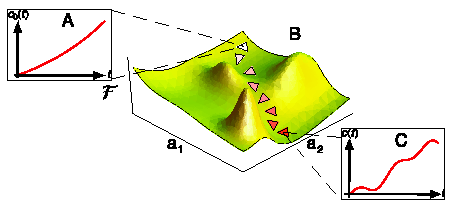
\includegraphics{images/nelder_mead}\\
      {\footnotesize\vspace{-2mm}\hspace{-15mm} Doria et al. PRL 106, 190501 (2011)}
  \end{center}
  \vspace{12pt}
  e.g. Nelder-Mead (simplex), genetic algorithms\dots
\end{frame}

\backupend

\end{document}
